\documentclass[11pt,a4paper]{article}
\usepackage[T1]{fontenc}
\usepackage[utf8]{inputenc}
\usepackage{lmodern}
\usepackage[margin=2.5cm]{geometry}
\usepackage{microtype}
\usepackage{amsmath,amssymb}
\usepackage{graphicx}
% src/eqm/source/styles/logo-ic-unicamp.sty

\ProvidesPackage{logo-ic-unicamp}
\RequirePackage{graphicx}

\newcommand{\LogoIcUnicampSize}{60pt}
\newcommand{\LogoIcUnicampFile}{logo-ic-unicamp.pdf}

\advance \endlinechar by -256 %

\def\LogoIcUnicampWidth{\LogoIcUnicampSize}    %
\def\LogoIcUnicampHeight{\LogoIcUnicampSize}   %

\newcommand{\LogoIcUnicampBare}{
  \hbox{\includegraphics*[width=\LogoIcUnicampWidth]{\LogoIcUnicampFile}}
}

\newcommand{\LogoIcUnicamp}{
  \vbox to \LogoIcUnicampHeight{
    \offinterlineskip
    \hrule height 0pt width 0pt depth 0pt
    \vss
    \LogoIcUnicampBare
    \vss
    \hrule height 0pt width 0pt depth 0pt
  }
}

\newcommand{\LogoIcUnicampFont}{
  \fontfamily{cmss}\fontseries{bx}\fontshape{n}\fontsize{7pt}{8pt}\selectfont
}

\newcommand{\LogoIcUnicampWithName}{
  \vbox to \LogoIcUnicampHeight{
    \offinterlineskip
    \hrule height 0pt width 0pt depth 0pt
    \kern 1pt
    \hbox to \LogoIcUnicampWidth{
      \hss
      \scalebox{0.82}{\hbox{\LogoIcUnicampBare}}
      \hss
    }
    \kern 1pt
    \hbox to \LogoIcUnicampWidth{
      \LogoIcUnicampFont {~}I\hss N\hss S\hss T\hss I\hss T\hss U\hss T\hss O\hss {~}\hss D\hss E{~}%
    }
    \vspace{0.1ex} %
    \hbox to \LogoIcUnicampWidth{
      \LogoIcUnicampFont {~}C\hss O\hss M\hss P\hss U\hss T\hss A\hss \c{C}\hss \~{A}O{~}
    }
    \kern 2pt
    \vss
  }
}

\advance \endlinechar by 256 %

\renewcommand{\LogoIcUnicampFile}{assets/branding/logo-ic-unicamp.pdf}
\usepackage[font=small,labelfont=bf]{caption}
\usepackage[section]{placeins}
\usepackage{booktabs,array,longtable,tabularx}
\usepackage[table]{xcolor}
\usepackage{listings}
\usepackage{tikz}
\usetikzlibrary{arrows.meta}
\definecolor{ReportNavy}{HTML}{071E47}
\definecolor{ReportCyan}{HTML}{0895A8}
\definecolor{ReportOrange}{HTML}{CC7100}
% Shared presentation for every table in the final report.
\definecolor{ReportTableStripe}{HTML}{F2F5F9}
\definecolor{ReportTableSubhead}{HTML}{E4ECF4}
\definecolor{ReportTableSummary}{HTML}{E3F1F3}
\definecolor{ReportTableRule}{HTML}{B9CDD9}
\definecolor{ReportTableText}{HTML}{253345}

\newcolumntype{L}{>{\raggedright\arraybackslash}X}
\newcolumntype{R}{>{\raggedleft\arraybackslash}X}
\newcolumntype{P}[1]{>{\raggedright\arraybackslash}p{#1}}

\newcommand{\ReportTableHead}{\rowcolor{ReportNavy}}
\newcommand{\ReportTableSubheadRow}{\rowcolor{ReportTableSubhead}}
\newcommand{\ReportTH}[1]{{\leavevmode\color{white}\bfseries\boldmath #1}}
\newcommand{\ReportSubTH}[1]{{\leavevmode\color{ReportNavy}\bfseries\boldmath #1}}
\newcommand{\ReportTableDivider}{\hline}
\newcommand{\ReportShape}[1]{\ensuremath{\mathsf{#1}}}

\NewDocumentEnvironment{ReportTable}{O{1.30} m +b}{%
  \begingroup
  \sffamily\small\color{ReportTableText}
  \renewcommand{\arraystretch}{#1}
  \setlength{\extrarowheight}{1.5pt}
  \setlength{\tabcolsep}{9pt}
  \setlength{\arrayrulewidth}{0.6pt}
  \arrayrulecolor{ReportTableRule}
  \rowcolors{2}{white}{ReportTableStripe}
  \begin{tabularx}{\linewidth}{#2}
    \noalign{\global\rownum=1}
    \showrowcolors
    #3
    \hiderowcolors
  \end{tabularx}
  \endgroup
}{}

\captionsetup[table]{font={small,sf},labelfont={bf,color=ReportNavy},
  justification=raggedright,singlelinecheck=false,skip=8pt}

\usepackage[hidelinks]{hyperref}
% Generated values come from config/project.toml via build.py.
\input{metadata.generated.tex}

\input{metrics.generated}
\graphicspath{{assets/final/}{../../slides/source/assets/}}
\setlength{\parindent}{1.2em}
\setlength{\parskip}{0.25em}
\setlength{\emergencystretch}{2em}
\renewcommand{\arraystretch}{1.15}
\renewcommand{\topfraction}{0.9}
\renewcommand{\bottomfraction}{0.8}
\renewcommand{\textfraction}{0.1}
\renewcommand{\floatpagefraction}{0.7}
\setcounter{topnumber}{3}
\setcounter{totalnumber}{4}
\lstset{language=Python,basicstyle=\ttfamily\footnotesize,
  keywordstyle=\color{ReportNavy}\bfseries,commentstyle=\color{black!60},
  frame=single,rulecolor=\color{black!20},breaklines=true,
  columns=fullflexible,keepspaces=true,showstringspaces=false,tabsize=4}
\hypersetup{pdftitle={\ProjectTitle: Final Project Report},pdfauthor={\ProjectAuthor},
  pdfsubject={MO809 final report: detection quality and computational scalability}}
\title{\ProjectTitle\\Under Perfect Communication\\[0.6em]\large Final Project Report}
\author{\ProjectAuthor\\\ProjectCourse}
\date{Presentation date: \FinalPresentationDate}

% Keep the front matter, main text, appendix, and references on recto pages.
% Inserted versos carry neither text nor page numbers.
\newcommand{\cleartorecto}{%
  \clearpage
  \ifodd\value{page}\else
    \hbox{}\thispagestyle{empty}\newpage
  \fi}

\begin{document}
\hypersetup{pageanchor=false}
\pagestyle{empty}
\begingroup
\thispagestyle{empty}
\centering
\color{black}

\noindent\begin{tabular}{ccc}
\raisebox{-.5\height}{
\includegraphics[width=2.2cm]{assets/branding/logo-unicamp.pdf}}
&
\begin{minipage}{0.6\textwidth}
\centering
{\sffamily\bfseries\fontsize{10}{14}\selectfont
 Universidade Estadual de Campinas\par
 Instituto de Computa\c{c}\~ao\par}
\end{minipage}
&
\raisebox{-.45\height}{\scalebox{1.11}{\LogoIcUnicampWithName}}
\end{tabular}\par
\vspace{0.6cm}

{\sffamily\bfseries\fontsize{11}{15}\selectfont\ProjectCourse\par}
\vspace{0.15cm}
{\sffamily\fontsize{10}{13}\selectfont 2s2026\par}
\vfill

{\sffamily\bfseries\fontsize{9}{12}\selectfont
 \textls[100]{FINAL PROJECT REPORT}\par}
\vspace{0.65cm}

{\bfseries\fontsize{23}{29}\selectfont
 \ProjectTitle\\Under Perfect Communication\par}
\vspace{0.80cm}

\rule{0.32\textwidth}{0.4pt}\par
\vspace{0.65cm}
{\sffamily\bfseries\fontsize{12}{15}\selectfont\ProjectAuthor\par}
\vfill

{\fontsize{10}{13}\selectfont
 Presentation date: \FinalPresentationDate\par}
\endgroup

\cleartorecto
\begingroup
\thispagestyle{empty}
\centering
\color{black}

{\sffamily\bfseries\fontsize{12}{15}\selectfont\ProjectAuthor\par}
\vspace{3.5cm}

{\bfseries\fontsize{23}{29}\selectfont
 \ProjectTitle\\Under Perfect Communication\par}
\vspace{1.6cm}

\begin{flushright}
\begin{minipage}{0.54\textwidth}
\small\raggedright
Final project report for the course
\ProjectCourse.
\par\vspace{0.45cm}
Professor: \ProjectProfessor.
\end{minipage}
\end{flushright}
\vfill

{\sffamily\fontsize{10}{13}\selectfont 2s2026\par}
\vspace{0.18cm}
{\fontsize{10}{13}\selectfont
 Presentation date: \FinalPresentationDate\par}
\endgroup

\cleartorecto
\pagenumbering{roman}
\pagestyle{plain}
\hypersetup{pageanchor=true}
\begingroup
\fontsize{11}{16}\selectfont
\setlength{\parindent}{0pt}
\setlength{\parskip}{10pt}
\section*{Abstract}
\addcontentsline{toc}{section}{Abstract}
Cooperative perception combines observations from several vehicles to reduce
the limitations of a single viewpoint, particularly when objects are occluded.
This project studies DiscoNet, a model that encodes local LiDAR observations,
aligns neighboring feature maps, and combines them through spatial attention
before predicting car detections. The experiments use a released pretrained
student network on V2X-Sim 2.0 under ideal communication and alignment, with no
retraining or checkpoint selection.

The detection benchmark evaluates the same model with feature sharing
disabled and enabled over 1,000 synchronized test frames and 4,000 active
vehicle views. Cooperation increases Average Precision (AP) from
\ReportOwnAPFifty\% to \ReportCoopAPFifty\% at an Intersection over Union (IoU)
threshold of 0.5, and from \ReportOwnAPSeventy\% to \ReportCoopAPSeventy\% at 0.7.
Because model weights remain fixed, this comparison measures the benefit of
enabling information sharing in the evaluated student.

A separate runtime experiment measures complete model execution for 1--20
input slots on a fixed 30-frame cohort. Recorded scans are replayed above
five inputs to increase computational load. A matched ablation then compares
the original complete collaboration graph with a coarse-attention maximum
spanning tree for 1--15 slots. The selected links restrict fine feature
fusion while retaining bidirectional exchanges and self contributions.
At 15 slots, the tree reduces median execution time by
\ReportTreeReduction\%, while AP decreases by \ReportTreeDropFifty\ and
\ReportTreeDropSeventy\ percentage points at IoU 0.5 and 0.7, respectively.

Together, the results show a detection benefit from feature sharing and a
concrete runtime--accuracy trade-off when collaboration is made sparse.
The analysis connects these measurements to DiscoNet's encoder, alignment,
attention, and decoder stages, distinguishing the information available to
each receiver from the computation required to process the group.
\par
\medskip
\begingroup
\raggedright
\noindent\textbf{Keywords:} Cooperative~perception; LiDAR; DiscoNet; V2X-Sim;
sparse~collaboration; runtime~scalability.
\par
\endgroup
\endgroup
\clearpage
\begingroup
\small
\setlength{\parskip}{0pt}
\tableofcontents
\endgroup
\clearpage
\phantomsection
\addcontentsline{toc}{section}{List of Figures}
\listoffigures
\cleartorecto
\pagenumbering{arabic}
\section{Introduction and Objectives}
An individual vehicle observes only part of its surroundings. Buildings,
other vehicles, sensor range, and viewpoint can hide objects that another
vehicle can see. Cooperative perception addresses this limitation by combining
information from multiple observers. The central question is which
information to exchange and how to use it without making computation and
communication costs impractical.

Figure~\ref{fig:occlusion} gives the motivating example used in the project
presentation. Vehicle A follows a truck and obtains returns from its rear
surface. Vehicle B has another line of sight and observes a car farther
ahead. Combining observations makes that complementary information
available to the receiver. This geometric example motivates cooperation;
DiscoNet implements it by exchanging features extracted from the observations.

\begin{figure}[htbp]
\centering
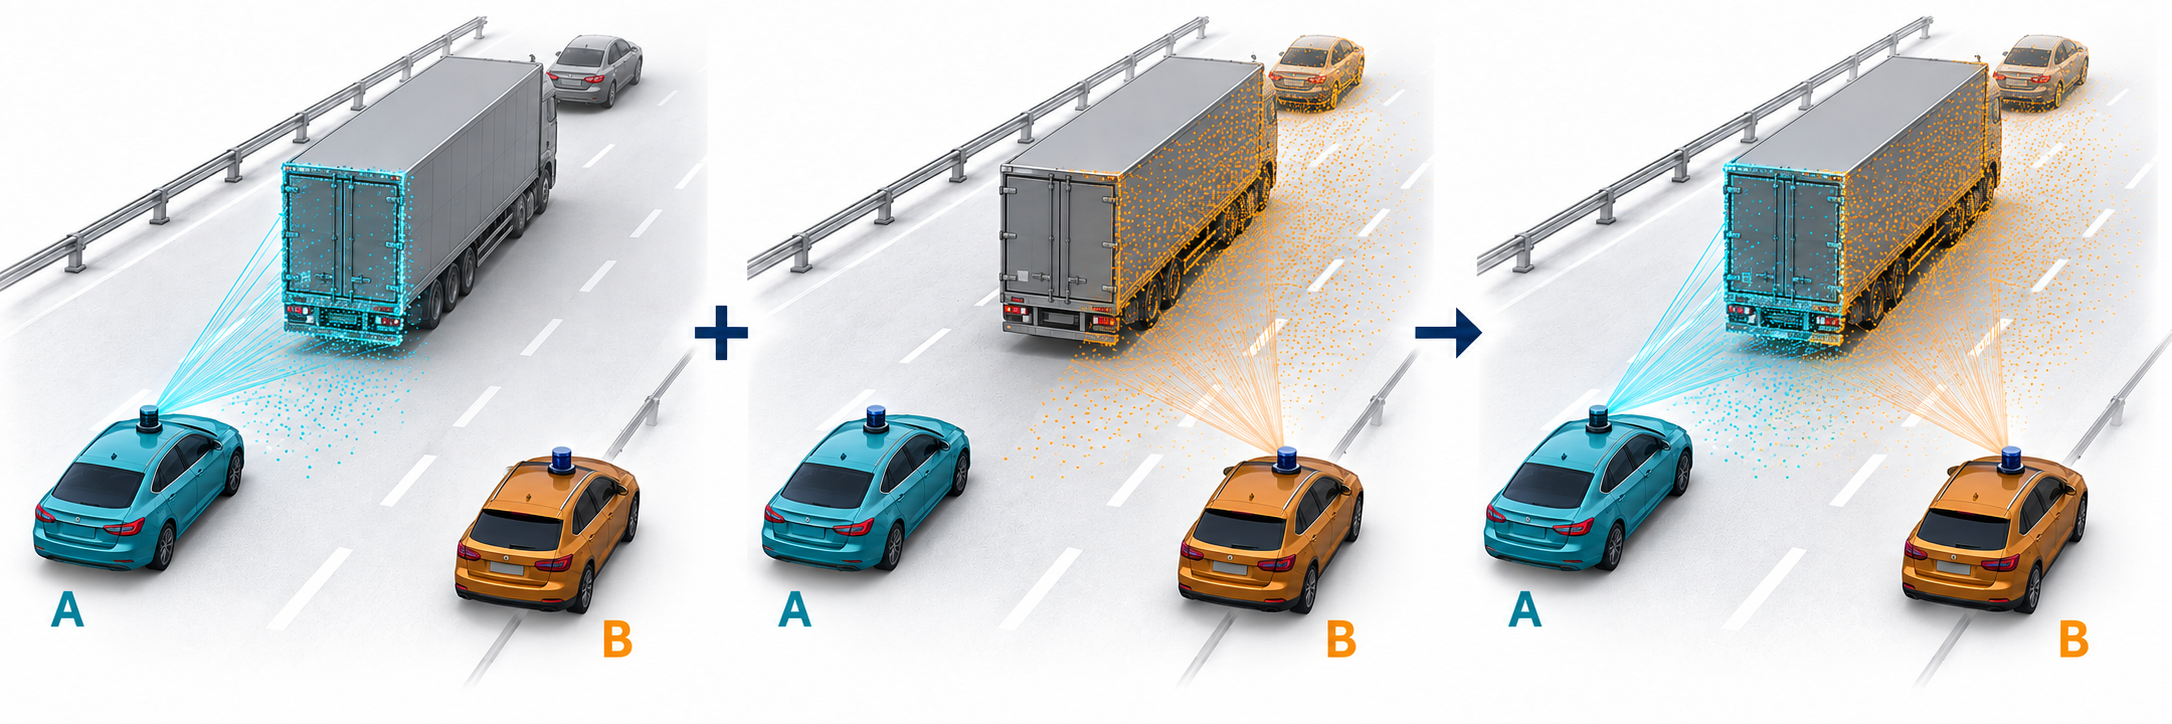
\includegraphics[width=\linewidth]{illustrations/lidar-cooperation-v2.png}
\caption[Complementary observations around an occluding truck]{Project
illustration of complementary LiDAR observations. Cyan and orange distinguish
the two observers; the final panel combines their information. The gray car
ahead of the truck is scene context in the first panel. This is the original
AI-assisted illustration used in the presentation.}
\label{fig:occlusion}
\end{figure}

DiscoNet, introduced by Li et al.~\cite{li2021disconet}, learns spatially
weighted collaboration between agents. This project examines that method
through its architecture and recorded evaluations, rather than developing or
training a detector from scratch. It addresses three questions:
\begin{enumerate}
  \item How are individual LiDAR observations transformed into cooperative
    object detections?
  \item How much does feature sharing improve detection for a fixed trained
    student under ideal communication?
  \item How does execution time grow with the number of model inputs, and
    what changes when fine-resolution collaboration is restricted to a tree?
\end{enumerate}

The original proposal planned a comparison of own-scan perception, early
fusion, and DiscoNet. The completed evidence supports a narrower accuracy
comparison: the same DiscoNet student is evaluated with information sharing
disabled and enabled. Early fusion is explained as the teacher's training
strategy, but no measured early-fusion baseline is available in these results.
The sparse-tree experiment is an additional inference-time ablation of the
released student; it introduces no new training or updated weights.

This study combines the architectural analysis and recorded evidence
presented in the final project slides~\cite{recordslides}. It specifies the
evaluation units and analyzes three distinct experiments. The
full-test benchmark measures detection quality across all active vehicle
views. A separate 30-frame workload measures runtime through 20 input slots.
A matched 30-frame Original/Tree experiment measures runtime and ego-vehicle
AP through 15 slots. These evidence sets are kept separate throughout.

\subsection{Scope and Communication Assumptions}
All conditions assume synchronized observations, accurate relative vehicle
poses, no packet loss, and no communication delay. Agents are evaluated on a
single computer with one GPU. Therefore, a model input slot represents an
agent's data within that computation, not a physically distributed process.
Measured runtime describes the implementation on the recorded hardware; it
does not include a wireless network or establish an end-to-end vehicle
communication latency.

\begin{figure}[htbp]
\centering
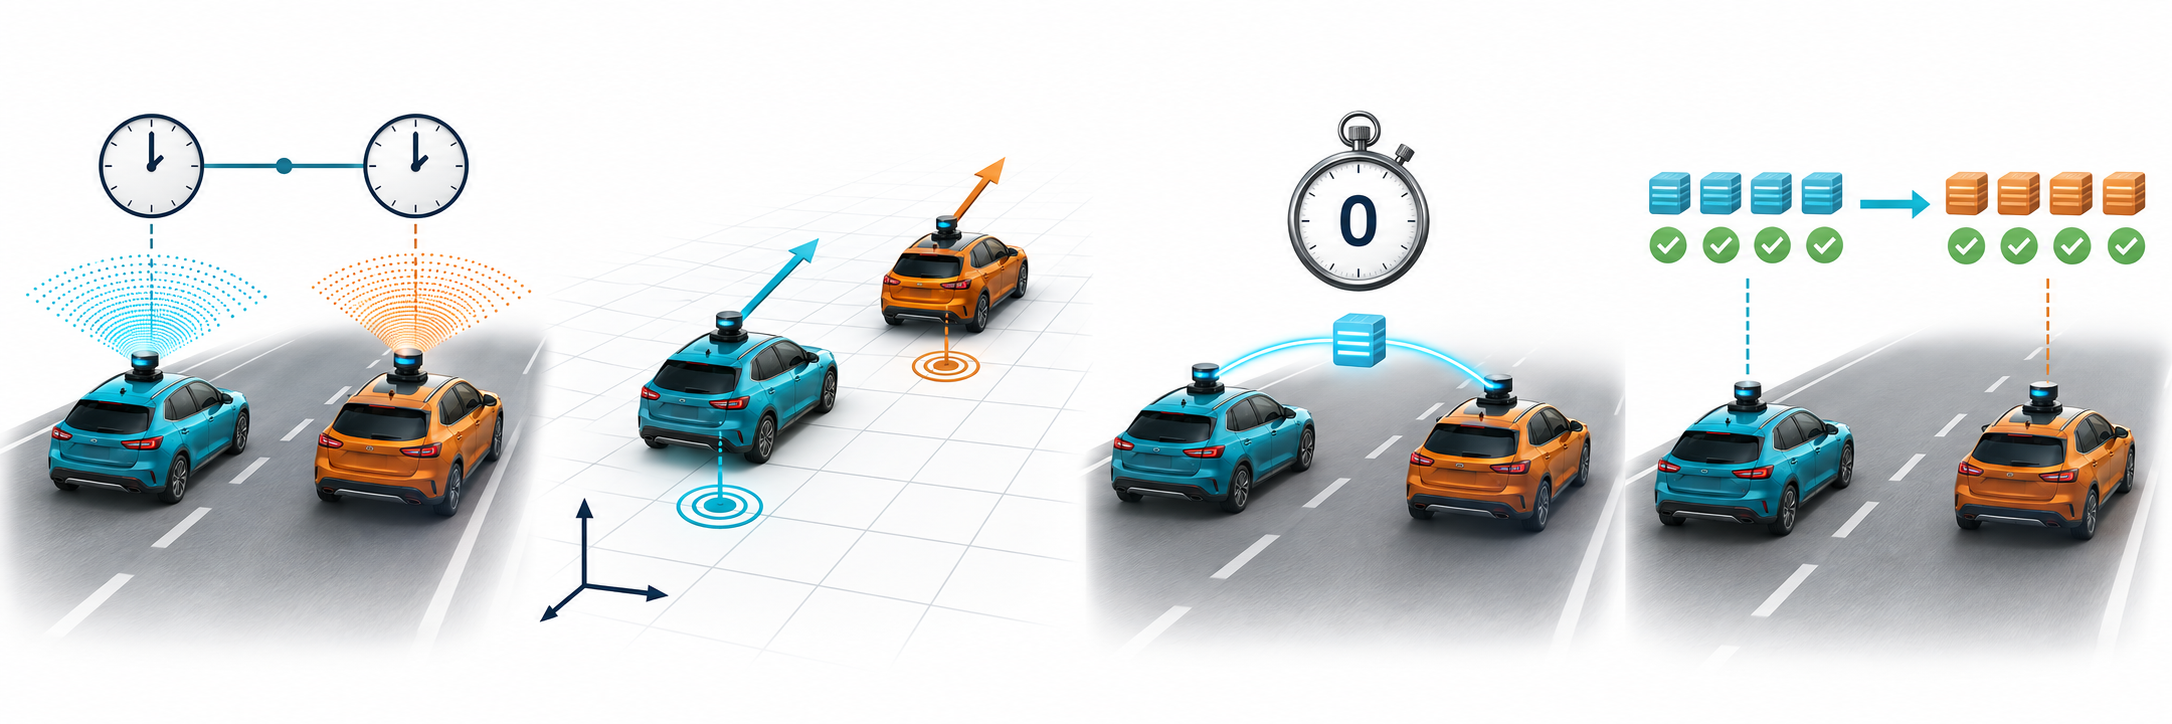
\includegraphics[width=\linewidth]{illustrations/perfect-communication.png}
\caption[The project's ideal communication assumptions]{Project illustration
of the four ideal conditions: synchronized observations, known poses,
zero assumed transmission delay, and complete packet delivery. The clocks,
poses, and packet symbols are explanatory artwork.}
\label{fig:communication-assumptions}
\end{figure}

Figure~\ref{fig:communication-assumptions} summarizes what perfect
communication means in this study. Synchronization makes observations
refer to the same instant, and relative poses allow their feature maps to
be expressed in one coordinate system. Complete delivery means the model
receives the selected inputs without dropped messages. Under these
conditions, the experiments can concentrate on feature fusion and its
computational cost.

\subsection{Organization and Visual Material}
The report follows the path from local observations to cooperative
detections, then explains how those detections and their execution cost
were evaluated. The architecture figures developed for the project expose
individual tensor transformations. The worked metric and convolution
examples make the numerical operations explicit. Recorded detection
overlays, camera views, and quantitative plots then connect that explanation
to the experiment evidence.

Existing project figures are reused throughout, including AI-assisted
conceptual illustrations and vector diagrams~\cite{recordfigures}. Captions
identify teaching examples and recorded results. The additional figure
snapshots and their source hashes are bundled with this report, so the
illustrated explanation remains available with the document sources.

\section{DiscoNet and Cooperative Feature Fusion}
\label{sec:method}
\subsection{Collaboration Strategies and Distillation}
Early fusion combines raw observations before feature extraction. Intermediate
fusion exchanges learned features, while late fusion combines detection
outputs such as boxes and scores. These choices place collaboration at
different stages of the perception pipeline.

\begin{figure}[htbp]
\centering
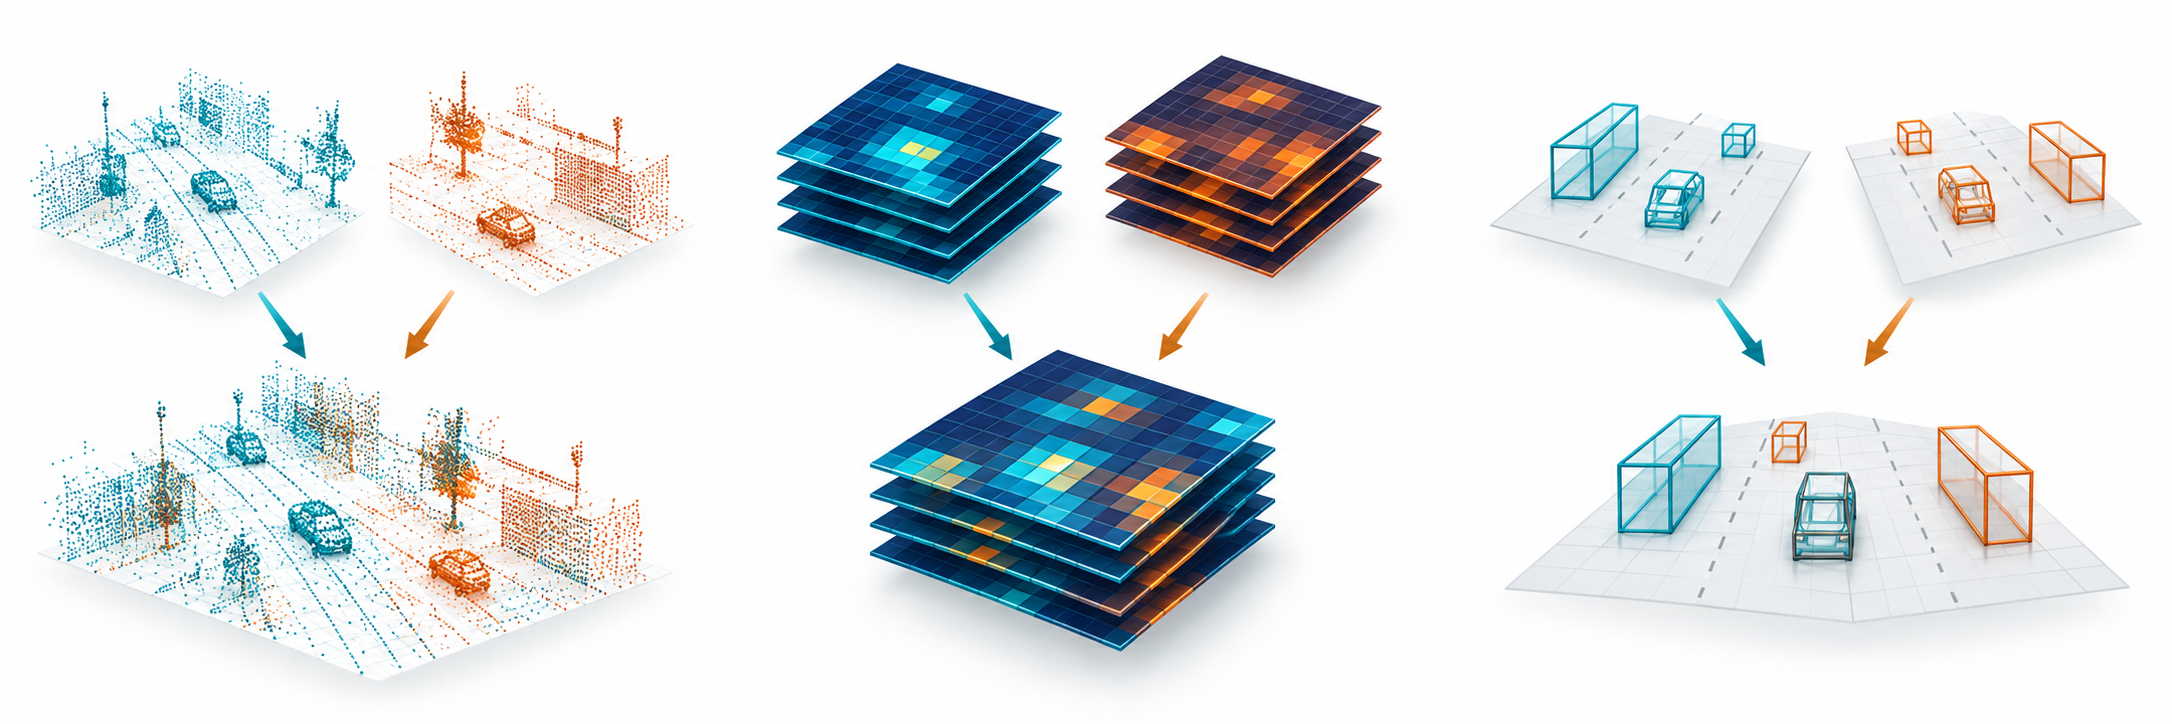
\includegraphics[width=\linewidth]{illustrations/fusion-strategies.png}
\caption[Early, intermediate, and late fusion]{The project's comparison of
raw-point, learned-feature, and detection-level combination. The colored
tensors and boxes are conceptual AI-assisted artwork.}
\label{fig:fusion-strategies}
\end{figure}

Figure~\ref{fig:fusion-strategies} makes the exchanged representation
explicit. Early fusion places information from different observers together
before encoding. Intermediate fusion lets each observer first encode its
own input. Late fusion moves collaboration after local predictions. This
ordering determines which processing is local and which information is
available when collaboration takes place.

DiscoNet uses an early-fusion teacher to guide an intermediate-fusion student
during training. The teacher has a more complete observation, while the
student receives local and shared features. Distillation encourages
correspondence between their learned representations. Only the student is
needed at inference~\cite{li2021disconet}. The evaluations in this report load
the released student checkpoint; the teacher and its distillation loss are
not run as part of the measured detection pipeline.

\begin{figure}[htbp]
\centering
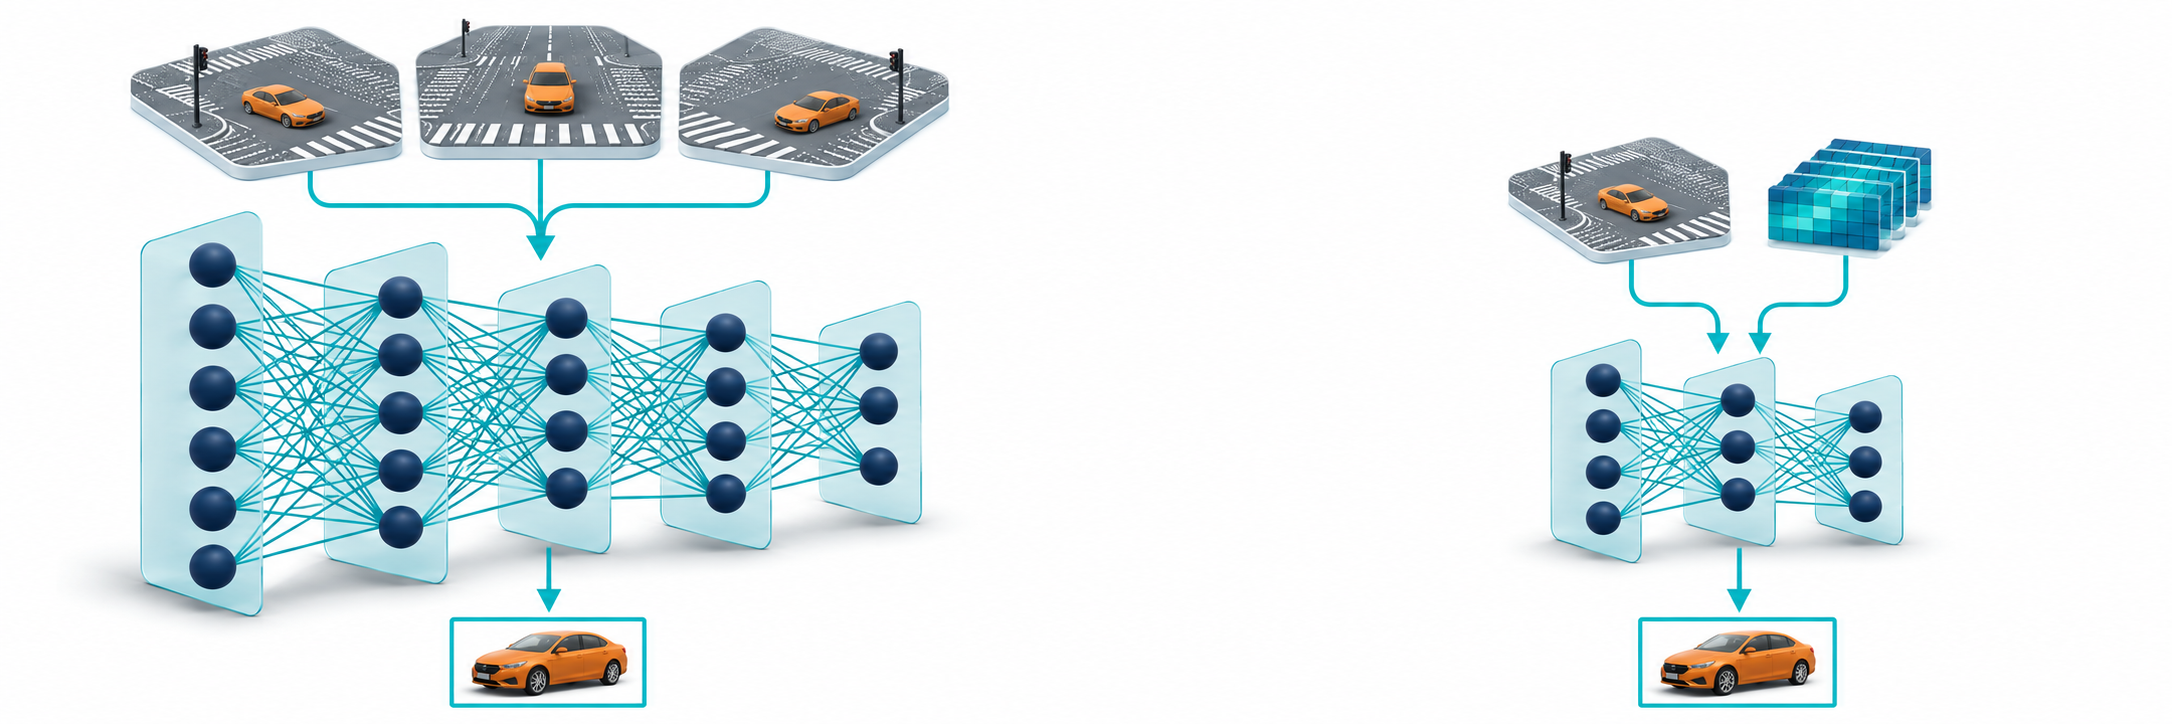
\includegraphics[width=0.92\linewidth]{illustrations/problem/problem-model-distillation-imagegen-v4.png}
\caption[Teacher guidance and the deployed student]{Project illustration
of teacher guidance and the student's detection task. Network sizes express
the teaching roles; the implemented teacher and student share the
encoder/decoder backbone.}
\label{fig:distillation}
\end{figure}

The training relationship in Figure~\ref{fig:distillation} is distinct from
the measured inference comparison. Turning sharing off restricts the same
student to its local scan. Turning sharing on provides peer features without
changing the checkpoint. The report therefore evaluates what collaboration
adds to that fixed student, rather than comparing a large teacher with a
separately trained smaller detector.

\FloatBarrier

\subsection{From LiDAR Points to Occupancy Grids}
The detector consumes the authors' prepared V2X-Sim 2.0 detection data.
CoPerception documents the preprocessing requirement and the availability of
prepared inputs~\cite{coperceptiondata}. The weekly technical material
describes the corresponding voxelization operation~\cite{recordslides}.
Invalid coordinates are rejected, and points near the sensor origin are
removed when both $-1<x<1$ and $-1<y<1$. Retained points satisfy
\[
  -32<x<32,\qquad -32<y<32,\qquad -3<z<2,
\]
with distances in meters. A binary occupancy grid uses horizontal cells of
$0.25\times0.25$ m and height bins of 0.4 m. The recorded model input has
shape $256\times256\times13$ in height--width--channels order: occupied cells
are set to one and cells without retained returns remain zero.
The reported runs start from prepared grids; raw-point preprocessing is not
part of their forward-runtime measurements.

\begin{figure}[htbp]
\centering
\begin{minipage}[c]{0.48\linewidth}
\centering
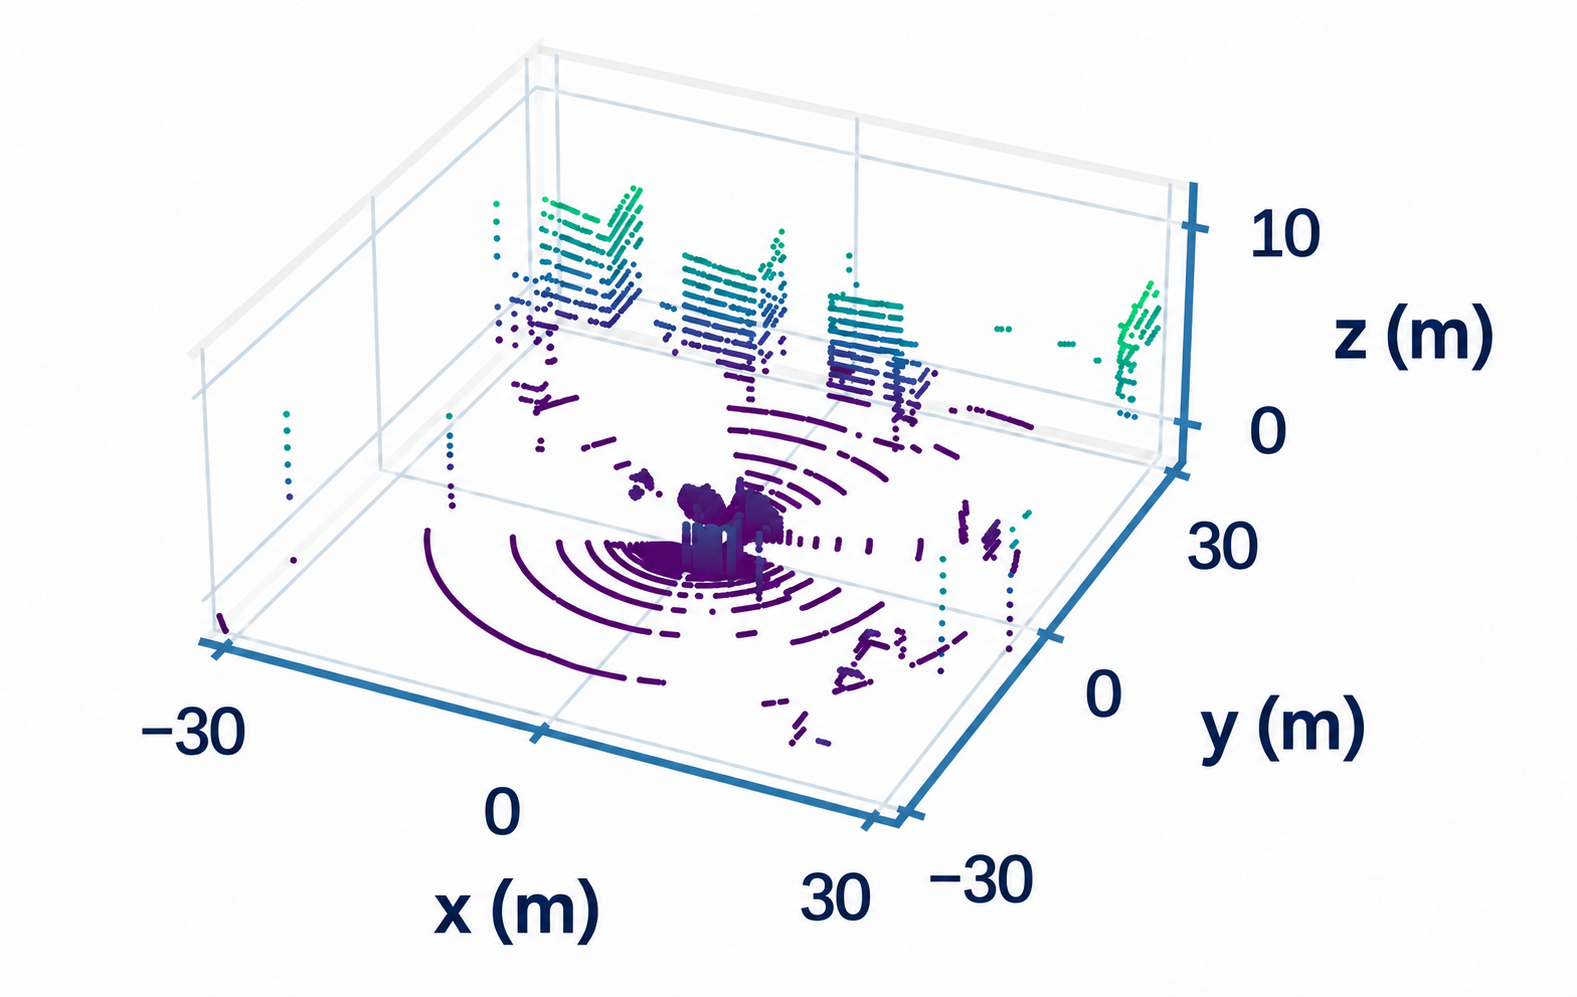
\includegraphics[width=\linewidth]{architecture/preprocessing/w44_raw_scan-imagegen-v3.png}
\small (a) A local LiDAR observation
\end{minipage}\hfill
\begin{minipage}[c]{0.48\linewidth}
\centering
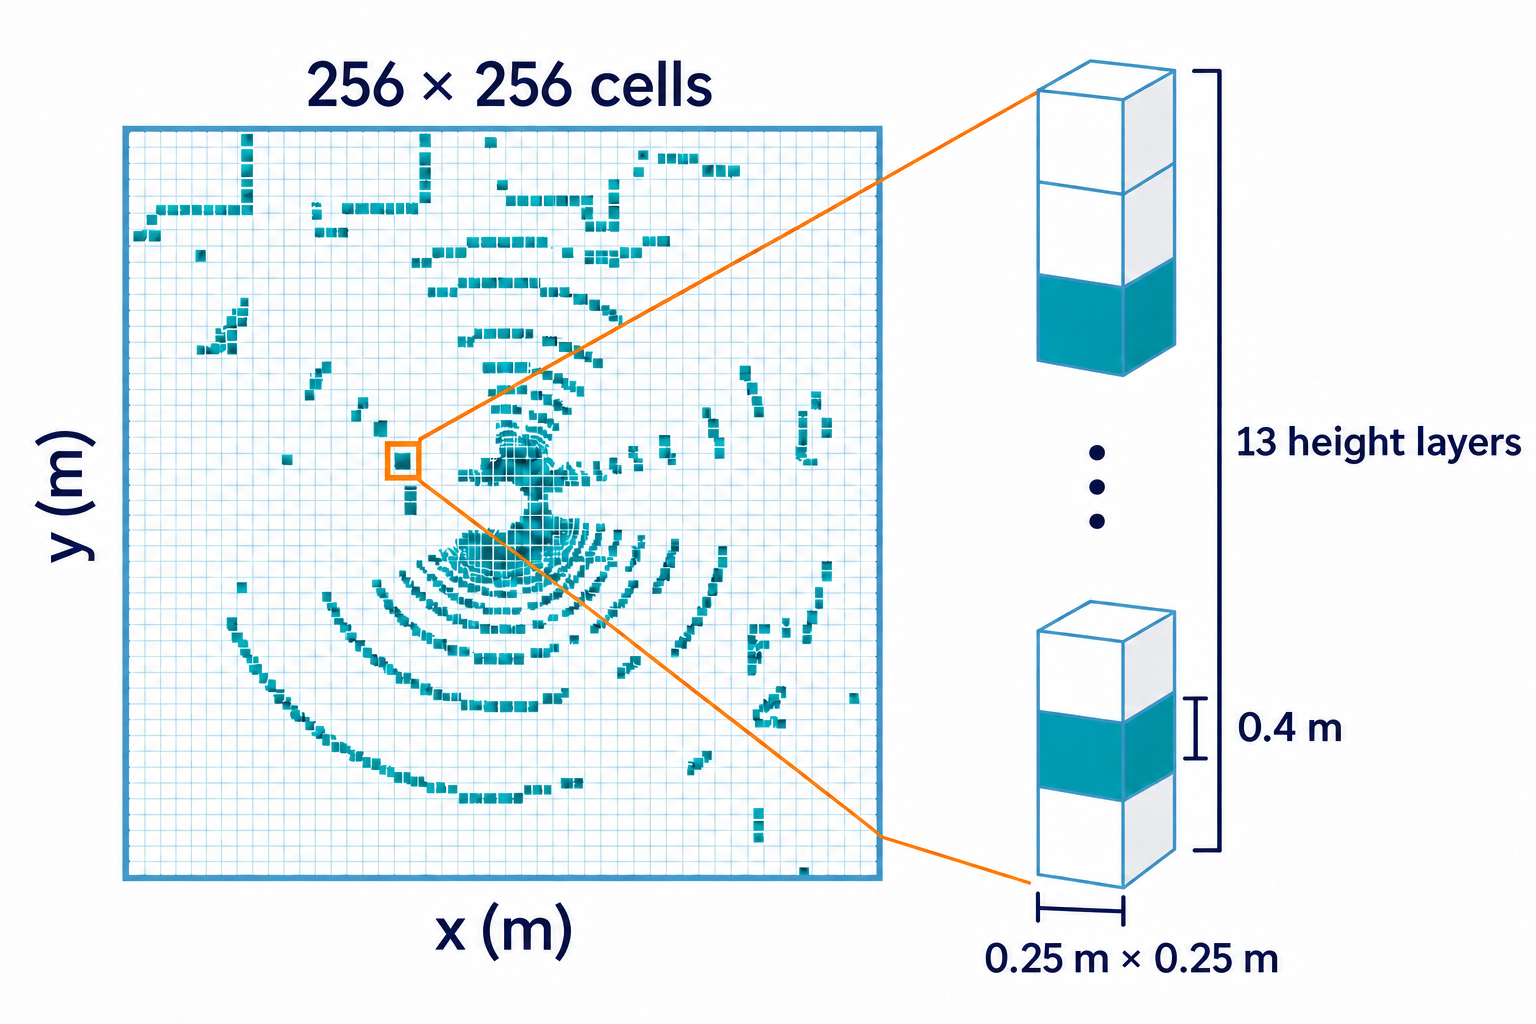
\includegraphics[width=\linewidth]{architecture/preprocessing/w44_occupancy_layers-imagegen-v3.png}
\small (b) Occupancy organized into height layers
\end{minipage}
\caption[From a local scan to occupancy height layers]{Project preprocessing
illustrations. Returns are assigned to spatial cells and height bins;
occupied cells have value one. These conceptual AI-assisted views explain
the representation rather than plotting a recorded input tensor.}
\label{fig:occupancy}
\end{figure}

The horizontal grid covers the 64-meter square around the sensor. Its
thirteen channels represent vertical occupancy bins; they are not thirteen
cameras or time steps. Figure~\ref{fig:occupancy} explains how height
information can enter a network that applies 2D spatial convolutions.
The layer stack is the channel dimension of the input feature tensor.

The diagrams use $H\times W\times C$ to make spatial size and channel
count visible. PyTorch stores 2D feature tensors in
$N\times C\times H\times W$ order. Batch and agent axes are omitted in
the illustrated shapes. These different display conventions describe the
same representation.

\FloatBarrier

\subsection{Reusable Units and the Encoder}
The architecture is assembled from a reusable 2D unit: a $3\times3$
convolution followed by batch normalization and ReLU. An Initial unit can
change channels while preserving spatial resolution; Keep preserves both;
Down uses stride two and doubles the channels. Figure~\ref{fig:encoder-units}
shows the unit and the encoder stage that composes these operations.

\begin{figure}[htbp]
\centering
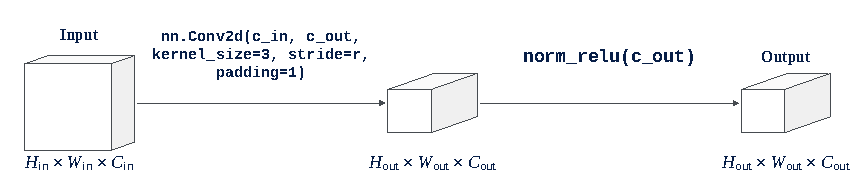
\includegraphics[width=\linewidth]{architecture/blocks/unit-2d-cubes-v4.pdf}\par
\vspace{0.6em}
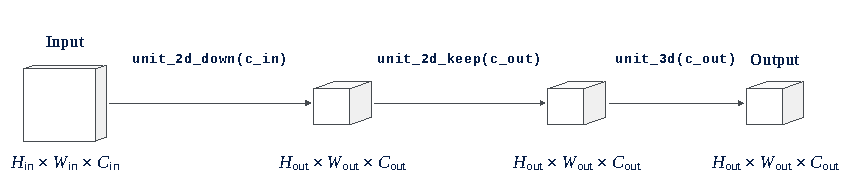
\includegraphics[width=\linewidth]{architecture/blocks/encoder-stage-cubes-v2.pdf}
\caption[The reusable 2D unit and encoder stage]{Project tensor diagrams:
the 2D unit above and its use inside an encoder stage below. The optional
pointwise 3D helper preserves the displayed spatial and channel dimensions.}
\label{fig:encoder-units}
\end{figure}

The optional 3D helper inserts a singleton depth axis, applies a
$1\times1\times1$ convolution, and flattens that axis again. Here it mixes
channels at each location rather than aggregating multiple recorded frames.
Appendix~\ref{app:implementation} contrasts this helper with a genuine
temporal convolution and gives the callable block definitions.

The encoder computes multiscale features independently for each vehicle.
Table~\ref{tab:architecture} summarizes the tensor routing shown in the
presentation. Batch and agent axes are omitted. The Stage 3 map is shared
with DiscoGraph, while the deeper Stage 4 output remains a local decoder
input. Saved encoder maps supply the decoder's skip connections.

\begin{table}[htbp]
\centering
\caption{Encoder feature shapes and routing. Tensor order is $H\times W\times C$.}
\label{tab:architecture}
\begin{ReportTable}{llL}
\ReportTableHead
\ReportTH{Stage} & \ReportTH{Output shape} & \ReportTH{Use} \\
Input & \ReportShape{256\times256\times13} & Prepared occupancy grid \\
0 & \ReportShape{256\times256\times32} & Saved for decoder Stage 8 \\
1 & \ReportShape{128\times128\times64} & Saved for decoder Stage 7 \\
2 & \ReportShape{64\times64\times128} & Saved for decoder Stage 6 \\
3 & \ReportShape{32\times32\times256} & Aligned and fused by DiscoGraph \\
4 & \ReportShape{16\times16\times512} & Local decoder input \\
\end{ReportTable}
\end{table}

\begin{figure}[htbp]
\centering
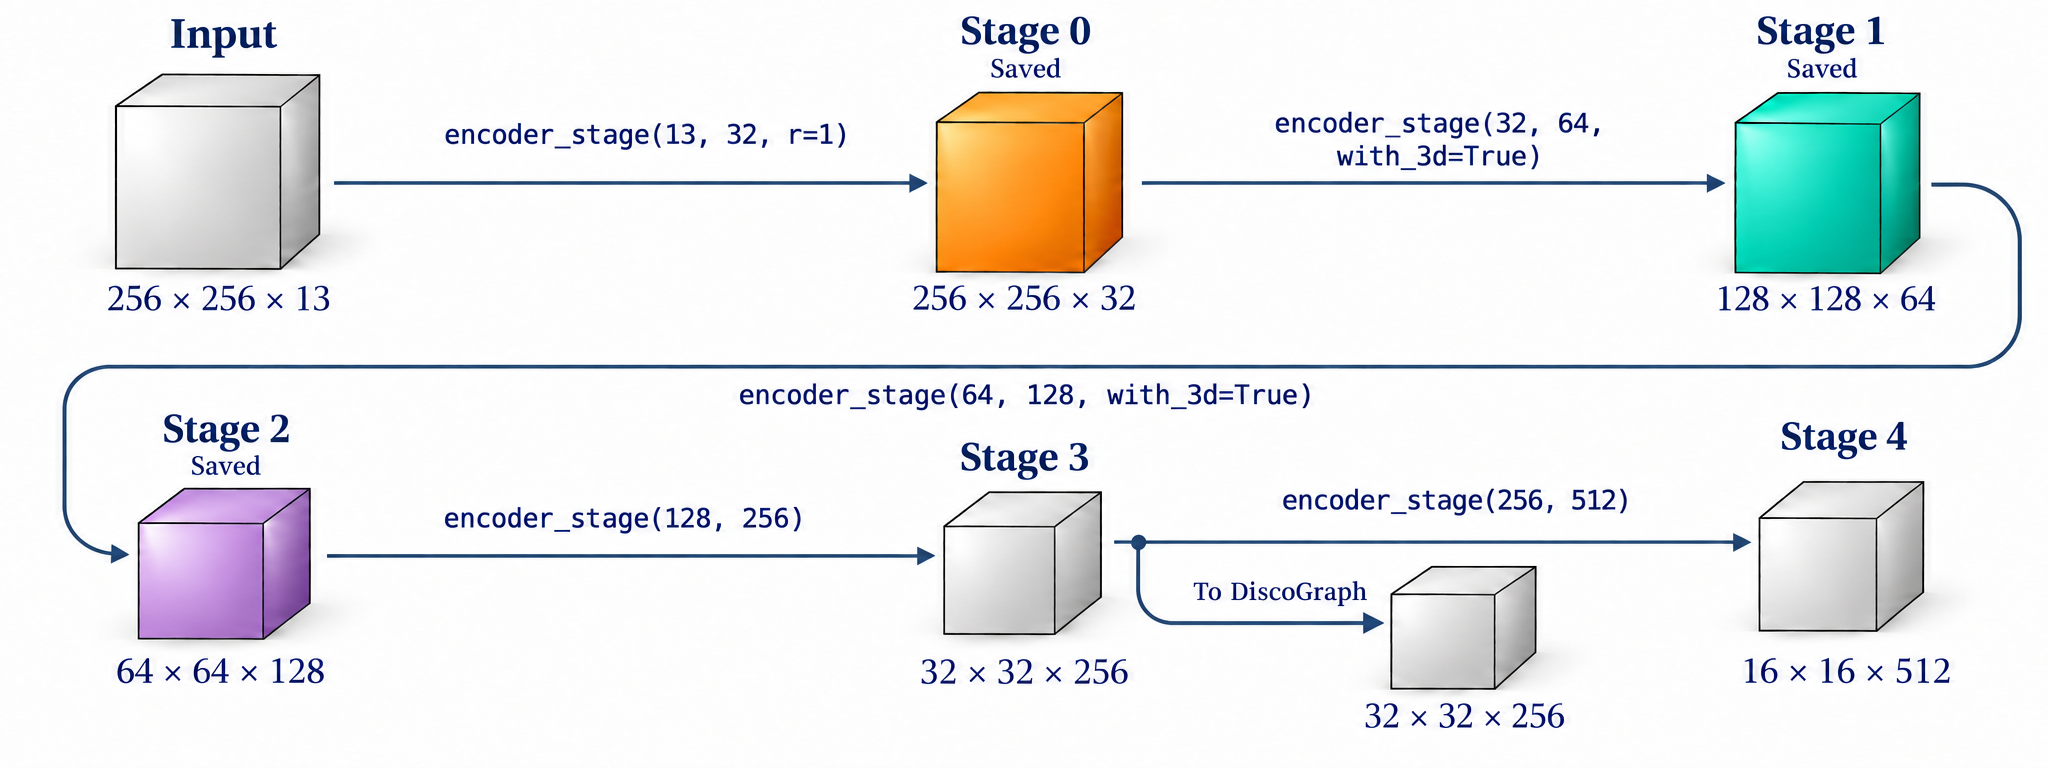
\includegraphics[width=\linewidth]{architecture/encoder/encoder-stage-pipeline-imagegen-v9.png}
\caption[Encoder tensor states and the collaboration branch]{Project encoder
pipeline illustration. Saved Stage 0--2 maps return through skip connections.
Stage 3 supplies the shared representation; Stage 4 supplies the deeper
local representation.}
\label{fig:encoder-pipeline}
\end{figure}

Spatial resolution falls as channel count increases in
Figure~\ref{fig:encoder-pipeline}. Collaboration acts on a $32\times32$
grid, with 256 channels at each location, rather than directly on the
$256\times256$ occupancy grid. The local Stage 4 path is retained alongside
this shared representation. The decoder will use both.

\FloatBarrier

\subsection{Spatial Alignment, Attention, and Fusion}
Let $F_u$ be sender $u$'s feature map and let $v$ be the receiving vehicle.
An alignment operator $\mathcal{T}_{u\to v}$ rotates and translates the
sender's map into the receiver's coordinates. It is based on their relative
poses, so the two maps describe the same physical region. In the recorded
implementation, feature resampling uses bilinear interpolation, zero padding,
and \texttt{align\_corners=False}~\cite{recordfulltest}.

\begin{figure}[htbp]
\centering
\begin{minipage}[c]{0.57\linewidth}
\centering
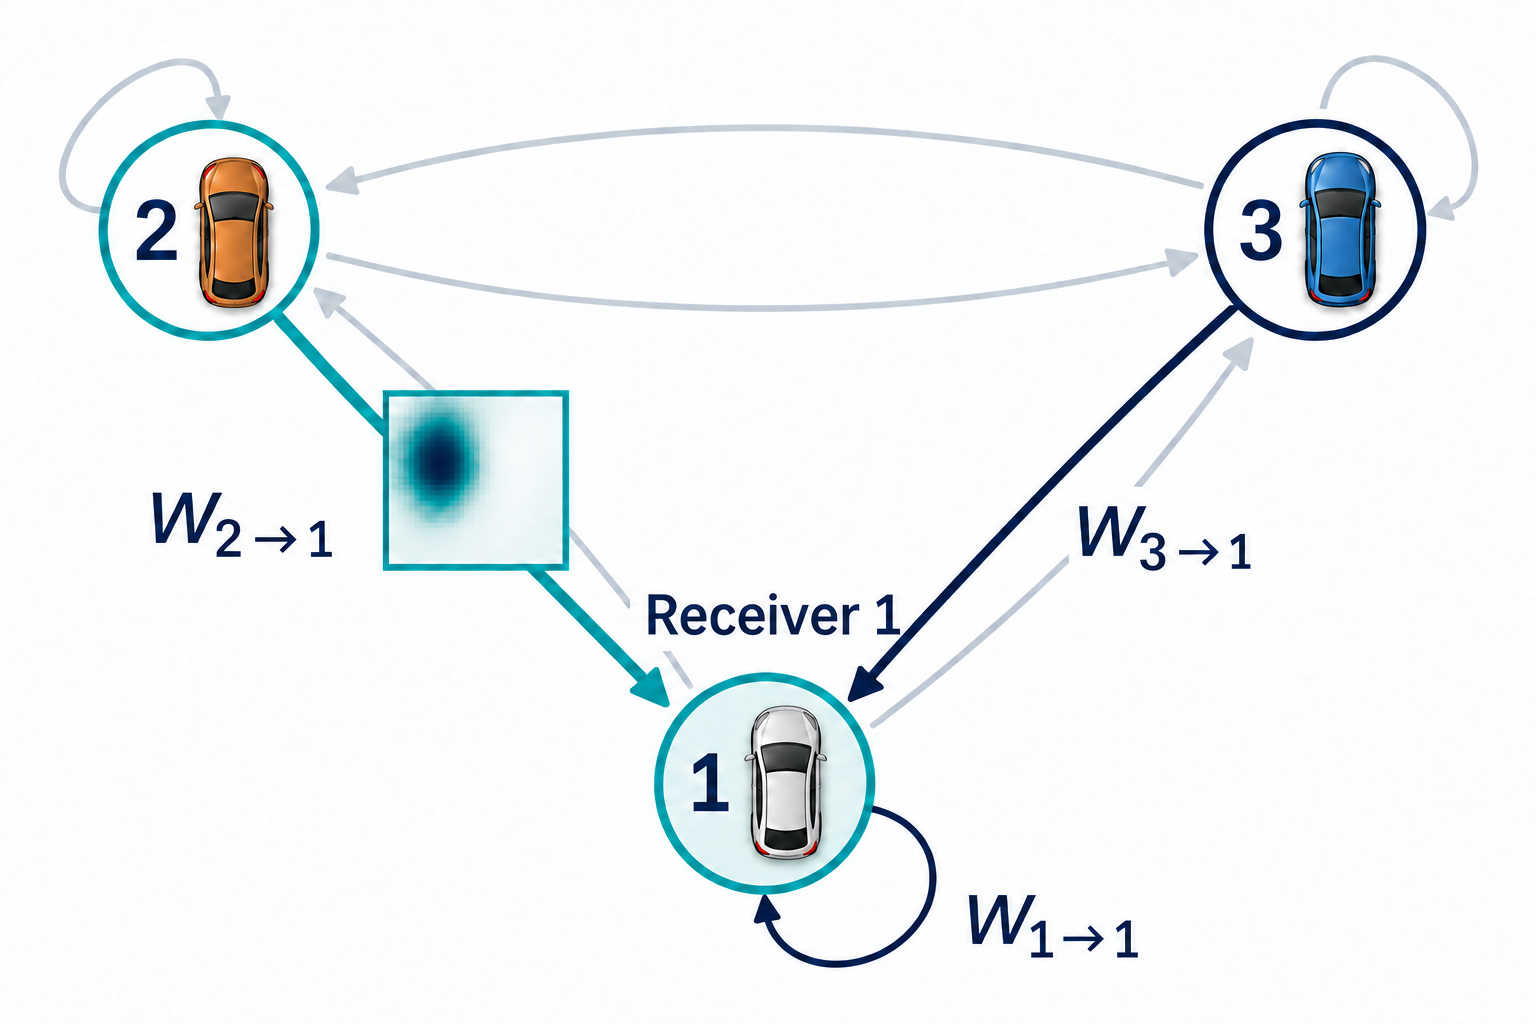
\includegraphics[width=\linewidth]{architecture/graph/discograph-three-agents-imagegen-v3.png}
\end{minipage}\hfill
\begin{minipage}[c]{0.39\linewidth}
\centering
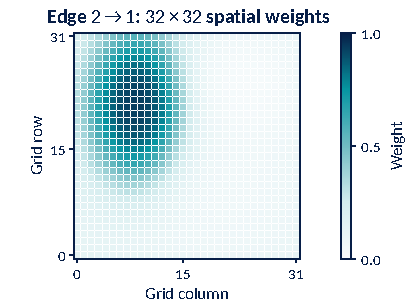
\includegraphics[width=\linewidth]{architecture/graph/discograph-three-agents-v2-spatial-map.pdf}
\end{minipage}
\caption[Directed interactions and a spatial edge-weight map]{The project's
three-agent teaching example. An edge carries a spatial weight map, so a
sender's influence can vary across the receiver's grid. Displayed weights
are synthetic examples.}
\label{fig:directed-graph}
\end{figure}

For $u\to v$, receiver $v$ defines the coordinate system. Reversing the
direction changes both the receiving grid and the feature pair being
scored. Equal array indices in two unaligned maps can refer to different
physical locations. Figure~\ref{fig:alignment} shows why corresponding
locations must be brought into agreement before their features are paired.

\begin{figure}[htbp]
\centering
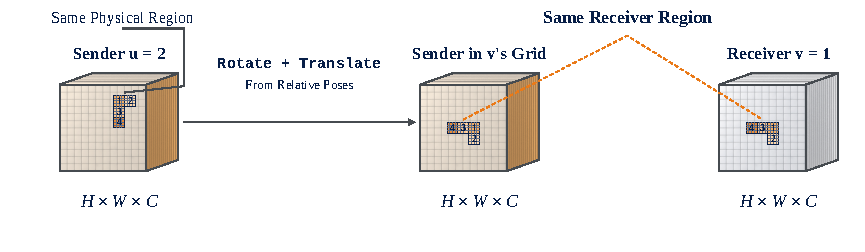
\includegraphics[width=\linewidth]{graph/discograph-step-01-alignment-v3.pdf}
\caption[Aligning sender features to the receiver's grid]{Project alignment
diagram. A pose-based transform moves the sender's representation into the
receiver's grid. The same spatial transform is applied to every channel.}
\label{fig:alignment}
\end{figure}

\begin{figure}[htbp]
\centering
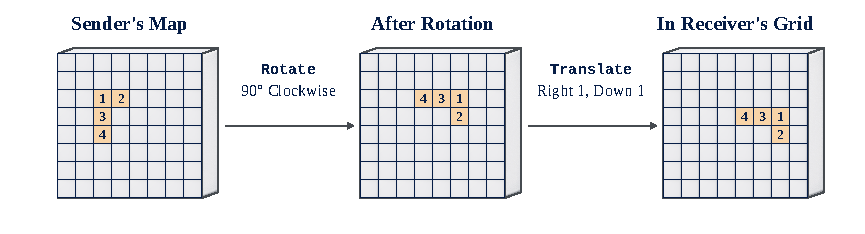
\includegraphics[width=\linewidth]{graph/discograph-rotation-translation-v3.pdf}
\caption[A worked rotation and translation on one feature channel]{The
project's $8\times8$ teaching example separates rotation from translation.
Colored cells track how a spatial pattern is relocated before fusion.}
\label{fig:rotation-translation}
\end{figure}

The small example in Figure~\ref{fig:rotation-translation} makes the
operation visible on one channel. Rotation changes the pattern's orientation;
translation changes its destination position. Feature channels remain
separate during this resampling. The sampling grid specifies where each
output cell reads the input, so output-to-input sampling uses the inverse
of a forward motion of points. The project's code example is included in
Appendix~\ref{app:implementation}.

\FloatBarrier
\subsection{Pairing Features and Computing Edge Scores}

The aligned sender features and receiver features are concatenated across
channels. A learned scoring function produces a spatial edge-score map,
\[
  s_{u\to v}(r,c)=g\!\left([F_v,\mathcal{T}_{u\to v}(F_u)]\right)_{r,c}.
\]
The implementation walkthrough reduces the paired channels through 128, 32,
and 8 intermediate channels before producing one score per spatial cell.

\begin{figure}[htbp]
\centering
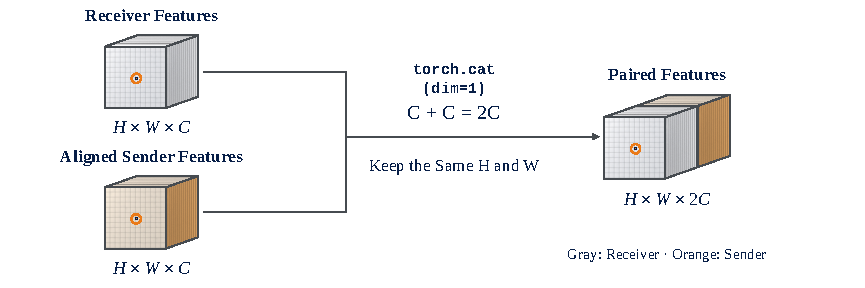
\includegraphics[width=\linewidth]{graph/discograph-step-02-pairing-v3.pdf}
\caption[Pairing receiver and aligned sender features]{Project diagram of
channel concatenation. Two 256-channel maps form a 512-channel pair at
each of the $32\times32$ collaboration locations.}
\label{fig:pairing}
\end{figure}

\begin{figure}[htbp]
\centering
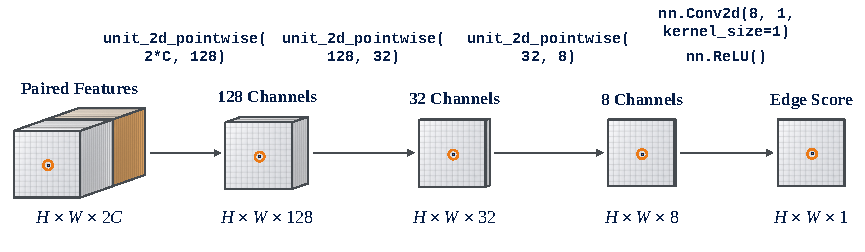
\includegraphics[width=\linewidth]{graph/discograph-step-03-scores-v4.pdf}
\caption[The edge-scoring subnetwork]{Project channel reductions from paired
features to an $H\times W\times1$ edge-score map. Spatial dimensions remain
unchanged while pointwise convolutions reduce the channel count.}
\label{fig:edge-scores}
\end{figure}

Concatenation preserves both input feature vectors rather than averaging
them. The pointwise scoring network then mixes their channels at each
location. Its final scalar describes that sender--receiver interaction
at one cell; it is distinct from the car-class confidence emitted later
by the detection head.

\FloatBarrier
\subsection{Spatial Weights and Feature Fusion}
A softmax across senders, including the receiver itself, gives
\begin{equation}
  a_{u\to v}(r,c)=
  \frac{\exp s_{u\to v}(r,c)}{\sum_{j=1}^{n}\exp s_{j\to v}(r,c)},
  \qquad \sum_{u=1}^{n}a_{u\to v}(r,c)=1.
\end{equation}

\begin{figure}[htbp]
\centering
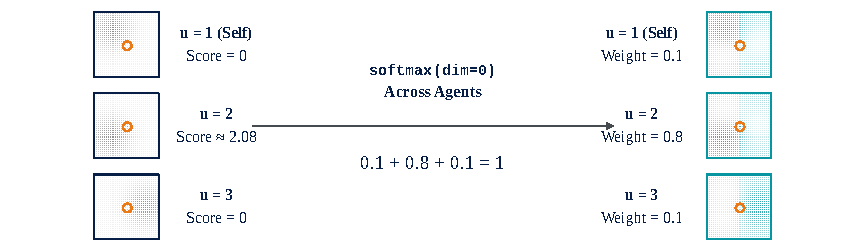
\includegraphics[width=\linewidth]{graph/discograph-step-04-softmax-v3.pdf}
\caption[Normalizing spatial weights across senders]{Project softmax
illustration. For one receiver and one cell, all contributing sender
weights sum to one. The operation is repeated across the spatial grid.}
\label{fig:spatial-softmax}
\end{figure}

Normalization acts on the sender axis, not on feature channels or on all
spatial cells together. Weights at two cells can therefore differ for the
same edge. A sender can have more influence in one region than another,
as the spatial map in Figure~\ref{fig:directed-graph} illustrates.

The fused map is
\begin{equation}
  \widetilde F_v(r,c,:)=
  \sum_{u=1}^{n}a_{u\to v}(r,c)\,
  \mathcal{T}_{u\to v}(F_u)(r,c,:).
\end{equation}
Thus, a scalar weight at a cell multiplies its entire channel vector, and
the weighted contributions are summed. The illustrated three-agent weights
in the presentation are teaching examples, not attention values measured
from these runs. Actual benchmark groups contain three to five active vehicles.

\begin{figure}[htbp]
\centering
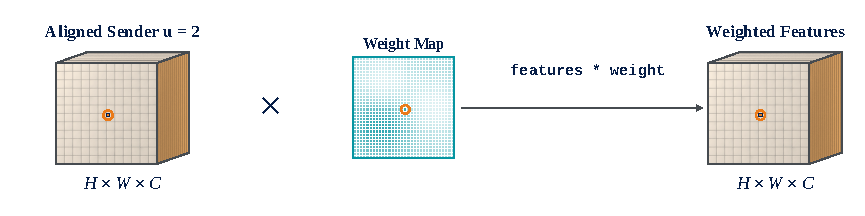
\includegraphics[width=\linewidth]{graph/discograph-step-05-weighting-v3.pdf}\par
\vspace{0.6em}
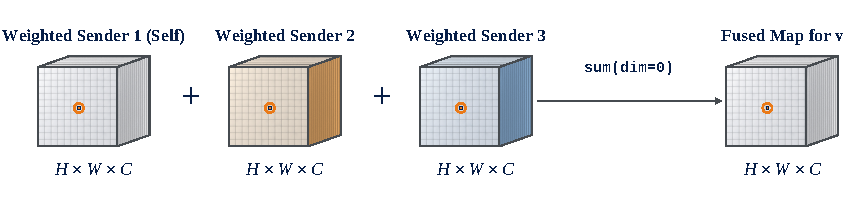
\includegraphics[width=\linewidth]{graph/discograph-step-06-fusion-v3.pdf}
\caption[Weighting contributions and summing the fused map]{Project diagrams
of the final operations. Above, a spatial scalar is broadcast over the
channel vector. Below, weighted maps, including the self contribution,
are added to form one fused map for the receiver.}
\label{fig:weighted-fusion}
\end{figure}

The fused output retains $H\times W\times C$. More senders add terms to
the sum rather than adding output channels. The self contribution keeps
the receiver's own representation in the same normalized competition as
its peer contributions. This completes one collaboration round.

\FloatBarrier
\subsection{Decoder, Skip Connections, and Detection Heads}
The first decoder stage upsamples the local Stage 4 output and concatenates
it with the fused Stage 3 map. Upsampling uses nearest-neighbor interpolation;
concatenation joins channels while matching spatial dimensions. Thus a
$16\times16\times512$ map becomes $32\times32\times512$ and is joined with
$32\times32\times256$ fused features, giving 768 channels.
Figure~\ref{fig:decoder-stage} exposes that sequence.

\begin{figure}[htbp]
\centering
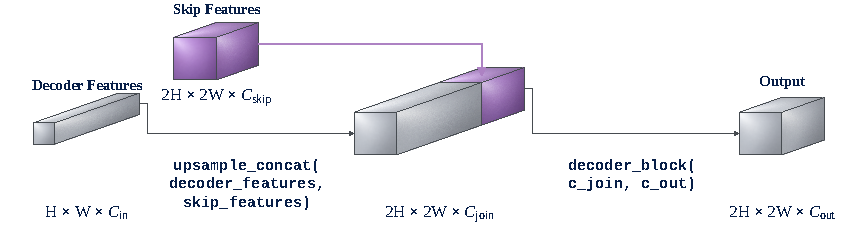
\includegraphics[width=\linewidth]{architecture/blocks/decoder-stage-cubes-v6.pdf}
\caption[Upsampling, skip concatenation, and the decoder block]{Project
decoder-stage diagram. Upsampling changes spatial size, concatenation
appends the skip channels, and the decoder block produces the next map.}
\label{fig:decoder-stage}
\end{figure}

Later stages use saved Stage 2, 1, and 0 features. Each skip already has the
target spatial resolution. The decoder block contains two 2D units with
stride one. Table~\ref{tab:decoder} records the channel arithmetic, and
Figure~\ref{fig:decoder-pipeline} shows the full route to the input grid size.

\begin{table}[htbp]
\centering
\caption{Decoder routing. All shapes use $H\times W\times C$.}
\label{tab:decoder}
\begin{ReportTable}{lLll}
\ReportTableHead
\ReportTH{Stage} & \ReportTH{Skip source} & \ReportTH{Concatenated shape} & \ReportTH{Output shape} \\
5 & Fused Stage 3 & \ReportShape{32\times32\times768} & \ReportShape{32\times32\times256} \\
6 & Saved Stage 2 & \ReportShape{64\times64\times384} & \ReportShape{64\times64\times128} \\
7 & Saved Stage 1 & \ReportShape{128\times128\times192} & \ReportShape{128\times128\times64} \\
8 & Saved Stage 0 & \ReportShape{256\times256\times96} & \ReportShape{256\times256\times32} \\
\end{ReportTable}
\end{table}

\begin{figure}[htbp]
\centering
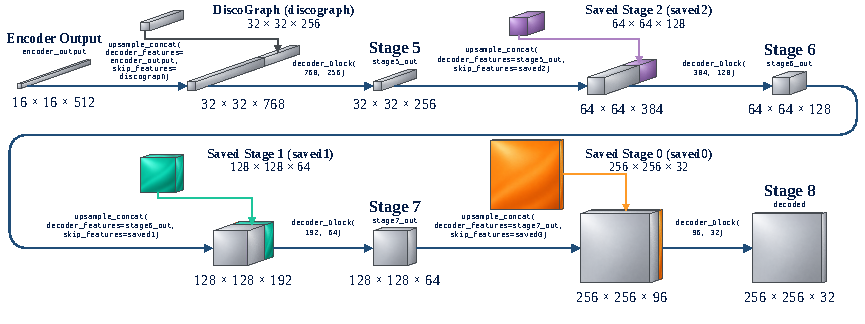
\includegraphics[width=\linewidth]{architecture/decoder/decoder-stage-pipeline-v6.pdf}
\caption[The complete decoder pipeline]{Project diagram of decoder
Stages 5--8. The first skip is the fused collaboration map; the other three
are saved local encoder maps. The output returns to $256\times256$ resolution.}
\label{fig:decoder-pipeline}
\end{figure}

The final $256\times256\times32$ map feeds classification and
box-regression heads. Classification produces background/car logits for
candidate anchors; regression produces box parameters. Decoding, confidence
filtering, and rotated NMS turn these dense outputs into the retained
detection set. Section~\ref{sec:metrics} explains its evaluation.

\subsection{Pairwise Work}
For $n$ active slots, the original complete graph evaluates $n^2$ ordered
sender--receiver pairs when self pairs are counted. There are $n(n-1)$ peer
pairs excluding self links. These are two conventions for the same graph,
not conflicting complexity claims. Pairwise collaboration contributes
quadratic work in $n$; the encoder, decoder, and heads also contribute to
the measured full-group execution time.

\section{Dataset and Experimental Protocol}
\subsection{V2X-Sim Release and Evaluation Units}
V2X-Sim provides simulated multi-agent observations and annotations for
collaborative perception~\cite{li2022v2xsim}. The source recordings include
vehicle and roadside sensors, but the experiments here exclude roadside-unit
inputs. Cameras provide visual context; they are not inputs to this LiDAR
detector. The official scene partitions and the recorded vehicle-only counts
are summarized in Table~\ref{tab:dataset}.

\begin{table}[htbp]
\centering
\caption{V2X-Sim 2.0 scene partitions used by the released detection protocol.}
\label{tab:dataset}
\begin{ReportTable}{Lrrrr}
\ReportTableHead
\ReportTH{Partition} & \ReportTH{Scenes} & \ReportTH{Frames} & \ReportTH{Vehicle inputs/frame} & \ReportTH{Vehicle scans} \\
Train & 80 & 8,000 & 2--5 & 29,200 \\
Validation & 10 & 1,000 & 3--5 & 4,000 \\
Test & 10 & 1,000 & 3--5 & 4,000 \\
\rowcolor{ReportTableSummary}
\textbf{Total} & \textbf{100} & \textbf{10,000} & --- & \textbf{37,200} \\
\end{ReportTable}
\end{table}

One synchronized frame contains observations from several active vehicles.
One \emph{vehicle view} is the output of one active vehicle at one frame.
The full test split contains 300 frames with three vehicles, 400 with four,
and 300 with five, giving 4,000 active views. Matching is performed within
each view; predictions are then pooled for AP. An object observed by two
vehicles contributes a reference box in each vehicle's evaluation view.
The 50,047 reference boxes in the benchmark therefore count view-specific
references, not unique physical cars across the recordings. The views are
also correlated observations, not 4,000 independent synchronized frames.

The original DiscoNet paper evaluates V2X-Sim 1.0, whereas this study uses
the prepared 2.0 detection release. CoPerception's documentation identifies
2.0 as its supported release~\cite{coperceptiondata}. The results are an
evaluation of that released implementation and checkpoint, not an exact
reproduction of the paper's 1.0 benchmark numbers.

\subsection{Model, Hardware, and Software}
All three experiments use the unchanged epoch-100 DiscoNet student in
float32 precision on one NVIDIA GeForce RTX 5060 Ti with approximately 16 GB
of GPU memory. The recorded setup has an AMD Ryzen 7 5700X CPU with eight
cores and sixteen threads, approximately 16 GB of system RAM, and Omarchy
Linux. The experiment environment records Python 3.14.8, PyTorch
2.9.1+cu128, and CUDA runtime 12.8.
The following results use this recorded configuration.

The checkpoint contains 15,843,505 parameters and is loaded with a strict
state-dictionary check. The inference implementation is pinned to source
commit \texttt{dd8fbb660300}. Its checkpoint hash and run identities are
stored with the evaluation records in the project repository.
No training, checkpoint selection, or parameter update is performed in the
reported evaluations.

\subsection{Detection Metrics and Postprocessing}
\label{sec:metrics}
Intersection over Union measures overlap between a prediction $B_p$ and
its reference box $B_g$:
\[
  \operatorname{IoU}(B_p,B_g)=
    \frac{|B_p\cap B_g|}{|B_p\cup B_g|}.
\]
AP is reported at matching thresholds of 0.5 and 0.7. The larger threshold
requires more accurate localization.

\begin{figure}[htbp]
\centering
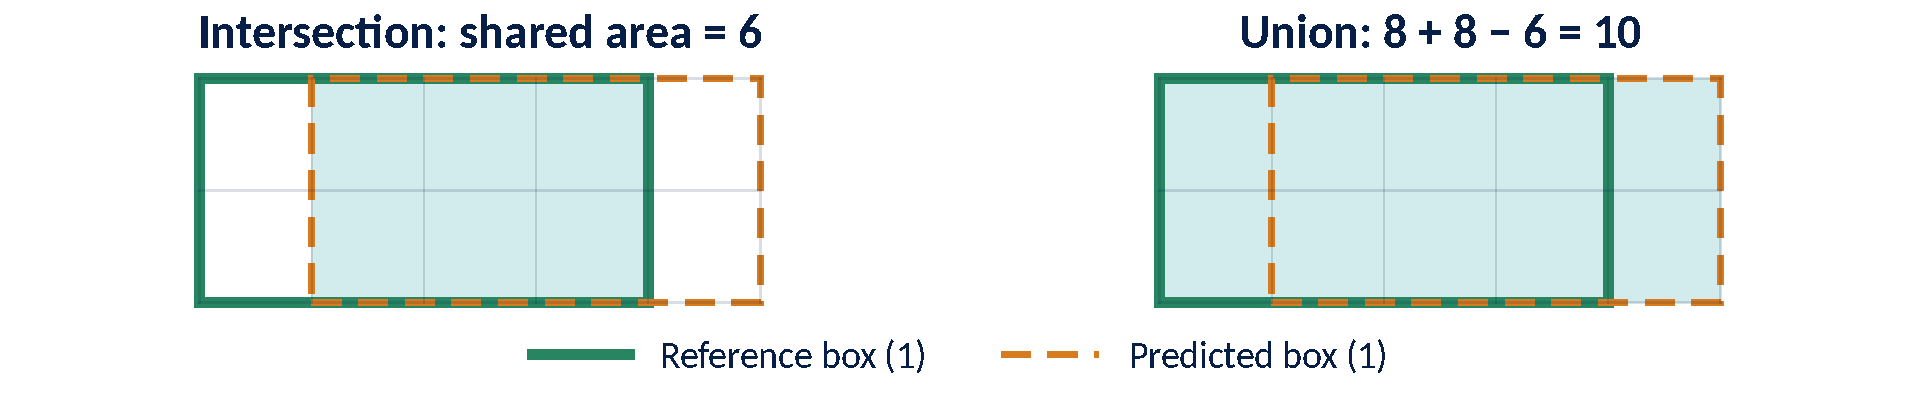
\includegraphics[width=\linewidth]{metrics/iou-overlap-v1.pdf}
\caption[Worked intersection and union areas]{Project IoU example. Both
rectangles have area eight, their intersection has area six, and their
union has area ten. The geometry is illustrative.}
\label{fig:iou-overlap}
\end{figure}

Figure~\ref{fig:iou-overlap} gives a concrete calculation:
\[
 \operatorname{IoU}=\frac{6}{8+8-6}=\frac{6}{10}=0.60.
\]
That prediction qualifies at a 0.5 matching threshold but fails at 0.7.
Figure~\ref{fig:iou-thresholds} extends the comparison to three overlaps.
The reference box is held fixed while the displacement of the prediction
changes. A stricter matching threshold asks for closer agreement with the
reference geometry.

\begin{figure}[htbp]
\centering
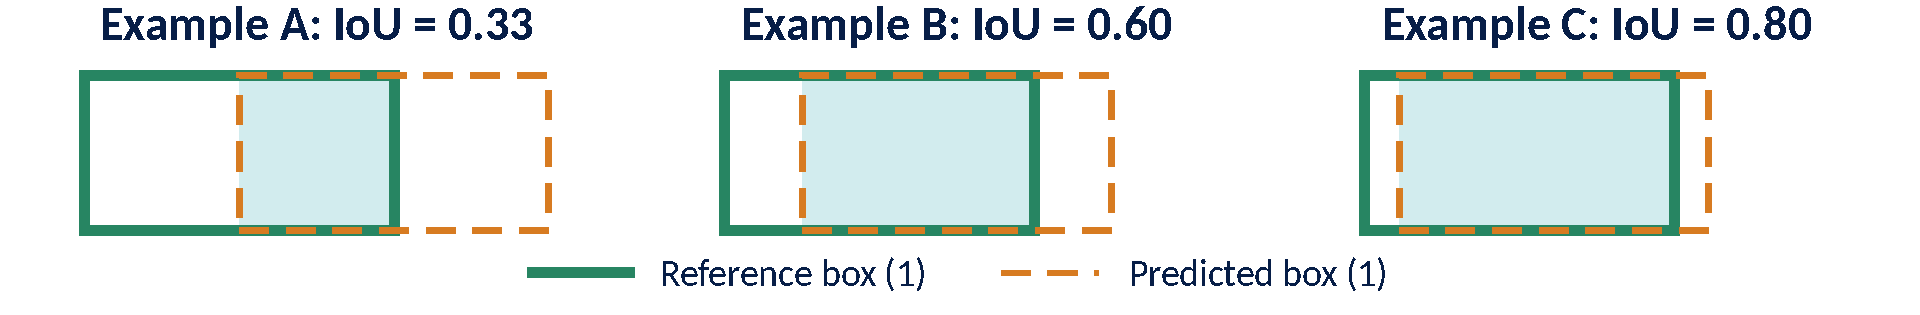
\includegraphics[width=\linewidth]{metrics/iou-thresholds-v1.pdf}
\caption[Three overlaps under the two matching thresholds]{Project geometry
examples with IoU approximately 0.33, 0.60, and 0.80. Only the last two
qualify at 0.5; only the last qualifies at 0.7.}
\label{fig:iou-thresholds}
\end{figure}

\FloatBarrier
\subsection{Confidence Scores and Retained Predictions}
The retained car score is obtained by a softmax of background and car logits:
\[
 p_{\mathrm{car}}=
 \frac{e^{z_{\mathrm{car}}}}{e^{z_{\mathrm{background}}}+e^{z_{\mathrm{car}}}}.
\]
The recorded evaluation keeps confidence strictly greater than 0.7 and uses
rotated nonmaximum suppression (NMS) with IoU 0.01. Confidence filtering
removes low-scoring candidates; NMS suppresses overlapping candidate
predictions. These operations precede matching to reference boxes.

\begin{table}[htbp]
\centering
\caption{The project's illustrative logits-to-confidence example.}
\label{tab:confidence-example}
\begin{ReportTable}{lRRRc}
\ReportTableHead
\ReportTH{Box} & \ReportTH{Background logit} & \ReportTH{Car logit} & \ReportTH{Car score} & \ReportTH{Score $>0.7$} \\
A & 1.0 & 3.0 & 0.881 & Keep \\
B & 2.0 & 1.0 & 0.269 & Discard \\
C & 1.0 & 4.0 & 0.953 & Keep \\
\end{ReportTable}
\end{table}

For Box A in Table~\ref{tab:confidence-example}, the conversion is
$e^3/(e^1+e^3)\approx0.881$. Box C ranks above A because its car score is
higher. Box B is removed by the confidence filter. These logits are the
worked example from the project slides, rather than outputs selected from
the benchmark.

Three thresholds have different jobs. The confidence threshold acts on a
class score. The NMS IoU threshold compares predictions with other
predictions. The evaluation IoU thresholds compare retained predictions
with reference boxes. Thus the score threshold of 0.7 and matching
threshold of 0.7 do not describe the same test.

\subsection{Precision, Recall, and Average Precision}
Predictions are ranked by their
car-class confidence, matched one-to-one within their vehicle view, and
classified as true positives (TP) or false positives (FP). Duplicate and
unmatched predictions are false positives. Precision and recall are
\[
  P=\frac{\mathrm{TP}}{\mathrm{TP}+\mathrm{FP}},\qquad
  R=\frac{\mathrm{TP}}{N_{\mathrm{reference}}}.
\]
AP integrates the interpolated precision envelope as recall increases.
It combines detection coverage and false-positive control; prediction count
alone is not AP.

Table~\ref{tab:ap-example} and Figure~\ref{fig:ap-example} reproduce the
project's four-prediction example with three reference cars. The first
prediction matches a reference. The second is a false positive, so recall
stays at $1/3$ and precision falls to $1/2$. The last two predictions match
the remaining references. Each reference can be credited only once.

\begin{table}[htbp]
\centering
\caption{Worked AP example with three reference cars and IoU matching at 0.5.}
\label{tab:ap-example}
\begin{ReportTable}{rrlRRR}
\ReportTableHead
\ReportTH{Rank} & \ReportTH{Score} & \ReportTH{Result} & \ReportTH{Cumulative TP / FP} & \ReportTH{Precision} & \ReportTH{Recall} \\
1 & 0.99 & TP & 1 / 0 & 100.0\% & 33.3\% \\
2 & 0.96 & FP & 1 / 1 & 50.0\% & 33.3\% \\
3 & 0.92 & TP & 2 / 1 & 66.7\% & 66.7\% \\
4 & 0.83 & TP & 3 / 1 & 75.0\% & 100.0\% \\
\end{ReportTable}
\end{table}

\begin{figure}[htbp]
\centering
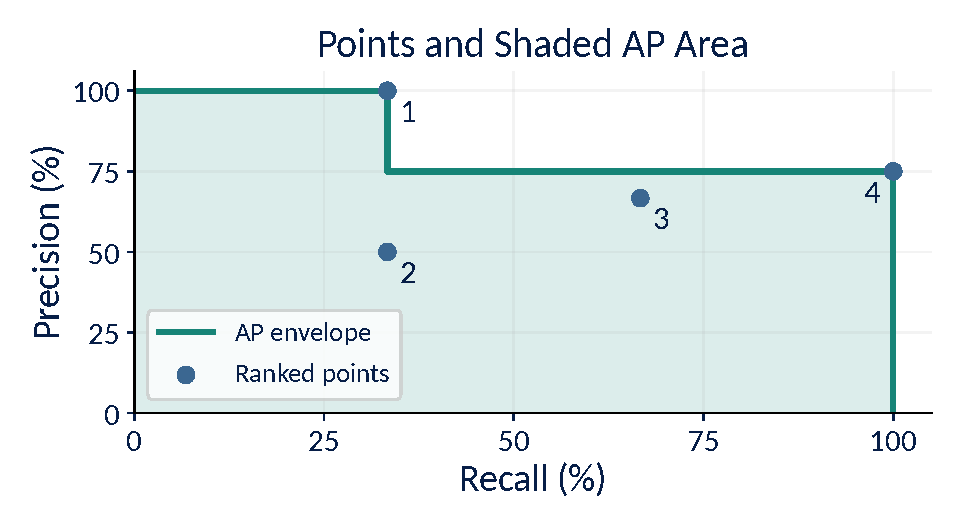
\includegraphics[width=0.76\linewidth]{metrics/ap-example-curve-v1.pdf}
\caption[A worked precision--recall curve and its envelope]{The project's
illustrative AP curve for Table~\ref{tab:ap-example}. The precision envelope
uses the best precision available at or beyond each recall level.}
\label{fig:ap-example}
\end{figure}

The interpolated envelope has precision one over the first third of recall
and $0.75$ over the remaining two thirds. Its area is
\[
 \operatorname{AP}=\tfrac13\times1+
                   \tfrac13\times0.75+
                   \tfrac13\times0.75
                 =\tfrac56\approx83.3\%.
\]
The false positive is present in the ranking even though every reference
eventually receives a match. Conversely, missed or filtered-out references
limit the maximum recall. The full-test curves in Section~\ref{sec:benchmark}
apply this evaluation to the recorded population rather than this small
teaching example.

\FloatBarrier

\subsection{Three Evidence Sets}
\label{sec:evidence-sets}
The full-test experiment compares sharing off and on over all 1,000 test
frames. The runtime-only experiment uses 30 fixed frames and measures
$n=1,\ldots,20$ slots without AP. The Original/Tree comparison uses 30 fixed
ego-1 views and measures both runtime and AP for $n=1,\ldots,15$.
The latter two use ten frames each from raw scenes \texttt{scene\_9},
\texttt{scene\_97}, and \texttt{scene\_98}. Their separately recorded timings
must not be substituted for one another. AP from the ego-only ablation is
also not directly comparable to AP pooled over all full-test vehicle views.

\begin{table}[htbp]
\centering
\caption{The three experiment populations and the questions they answer.}
\label{tab:evidence-sets}
\begin{ReportTable}{P{0.18\linewidth}P{0.28\linewidth}L}
\ReportTableHead
\ReportTH{Evidence set} & \ReportTH{Population} & \ReportTH{Reported outputs} \\
Full test & 1,000 synchronized frames; 4,000 active vehicle views &
  AP and fixed-checkpoint loss with sharing off/on \\
Runtime sweep & 30 recorded frames; 1--20 input slots &
  Full-group forward median and P95; no AP \\
Original/Tree & 30 ego-1 views; 427 reference cars; 1--15 slots &
  Matched forward medians and ego-view AP for both methods \\
\end{ReportTable}
\end{table}

Table~\ref{tab:evidence-sets} gives the denominator for each result before
the numerical comparisons. A synchronized frame, a vehicle view, an input
slot, and a timed forward are different units. Repeating a forward yields
another runtime sample, while repeating a scan in another slot changes the
computational workload. Neither operation creates a new independent
reference scene.

\section{Full-Test Detection Benchmark}
\label{sec:benchmark}
\subsection{Comparison and Results}
The benchmark evaluates the same pretrained student twice. In \emph{own scan
only}, a vehicle's prediction uses only its local observation and sharing is
disabled. In \emph{cooperative perception}, the student also uses aligned
features from the other active vehicles. Holding weights fixed isolates the
effect of enabling collaboration in this model. It does not compare two
separately trained detectors, and own scan only is not the paper's separately
trained lower-bound baseline.

Table~\ref{tab:full-test} contains the complete-split results from the saved
benchmark. Cooperation raises AP by
\ReportGainFifty\ percentage points at IoU 0.5 and \ReportGainSeventy\ points
at IoU 0.7. Improvements at both thresholds show that the gain is not
restricted to lenient box overlap in this evaluation.

\begin{table}[htbp]
\centering
\caption{Detection AP on 1,000 test frames and 4,000 active vehicle views.
Both conditions use the same epoch-100 weights.}
\label{tab:full-test}
\input{full-test-table.generated}
\end{table}

\begin{figure}[htbp]
\centering
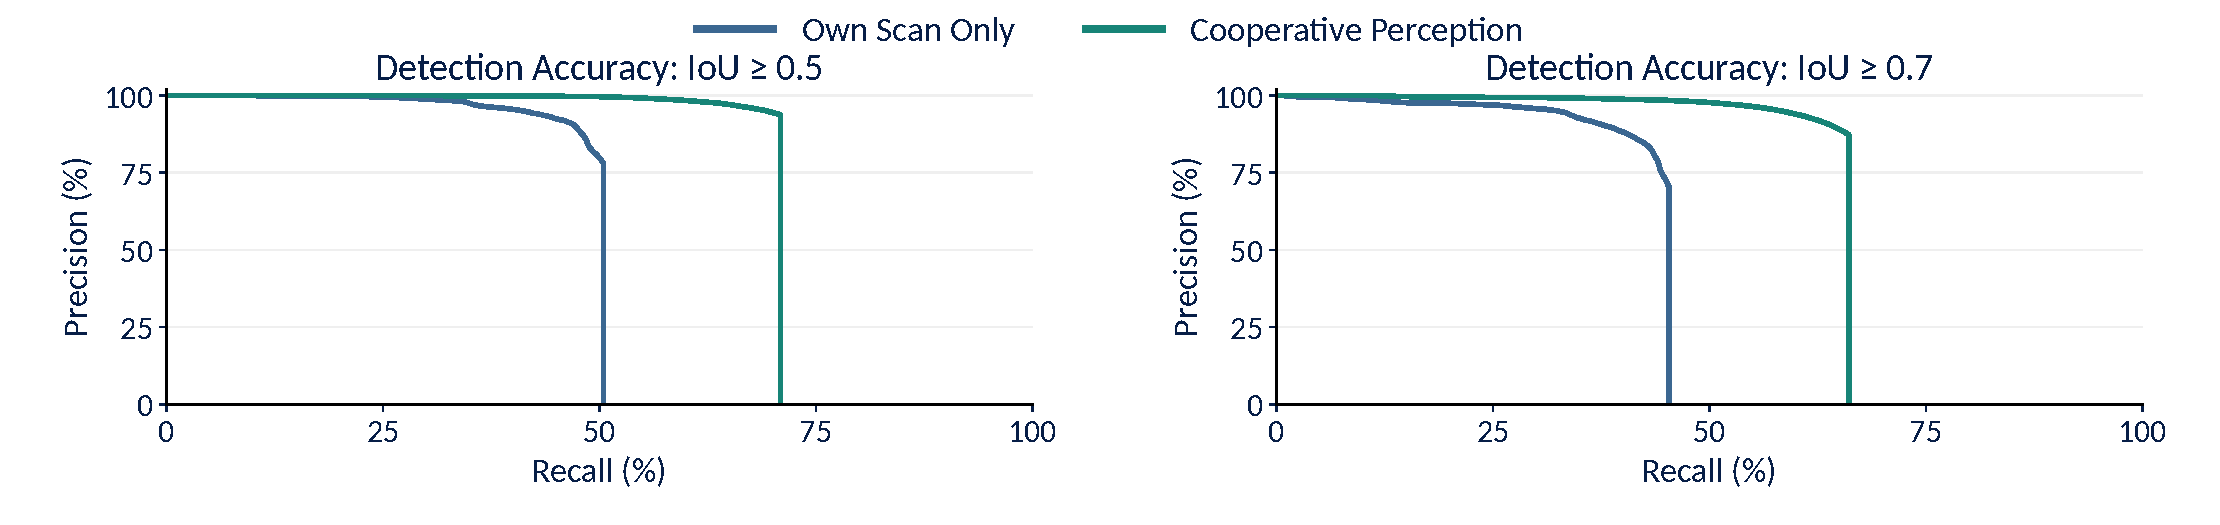
\includegraphics[width=\linewidth]{experiments/w45-2026-11-04/results-plots-v1.pdf}
\caption[Recorded full-test precision--recall curves]{Recorded full-test
precision--recall curves at IoU 0.5 and 0.7.
The curves and plotted values are reused from the saved evaluation, without
new inference or redrawing of the measured data.}
\label{fig:pr}
\end{figure}

The reproduced cooperative scores are approximately 70.4120\% and
64.8237\%. The archived audit compares these with the maintainer's checkpoint
log, 70.4136\% and 64.8239\%, respectively; the discrepancies are below
0.002 percentage points. The documentation table instead lists 69.03\% and
63.44\%. Agreement with the checkpoint log should not be described as
agreement with every published reference table, nor as replication of the
original paper's different-release benchmark.

The saved all-active-view accounting and the authors' collection policy give
identical AP and omit no active views. The record also reports exact
self-only output parity and selected postprocessing parity checks. These
checks support the implementation comparison, but do not establish robustness
to other datasets, checkpoints, or communication conditions.

\subsection{Fixed-Checkpoint Test Loss}
The supplementary record reports classification, box-localization, and total
test loss. Table~\ref{tab:loss} gives the unrounded-source
values displayed to two decimals. The original test code sums loss across
five padded vehicle slots, divides by five, and then averages across
synchronized frames. Inactive slots contribute zero. Thus these values
must be interpreted with that normalization rather than as loss per active
vehicle or a count of incorrect detections.

\begin{table}[htbp]
\centering
\caption{Mean fixed-checkpoint test loss under the authors' normalization.
No teacher or distillation term is included during evaluation.}
\label{tab:loss}
\input{loss-table.generated}
\end{table}

All three loss values are lower with collaboration, consistent with the AP
comparison. This is one evaluation of a fixed checkpoint, not a training
curve, learning-speed comparison, or reconstruction of validation history.
The loss and AP records therefore answer related but different questions.

\subsection{Qualitative Detection Example}
Figure~\ref{fig:detections} shows ego vehicle 1 in raw \texttt{scene\_5},
frame \texttt{000066}, with five participating vehicles. This example comes
from the recorded validation scene, not the 1,000-frame test benchmark.
Within the ego crop, there are 17 reference car boxes. Own scan only produces
11 predictions, while cooperation produces 17. At IoU at least 0.5, the
predictions match 10 and 16 reference cars, respectively.
Equal prediction and reference counts in the cooperative
case therefore do not mean perfect matching.

\begin{figure}[htbp]
\centering
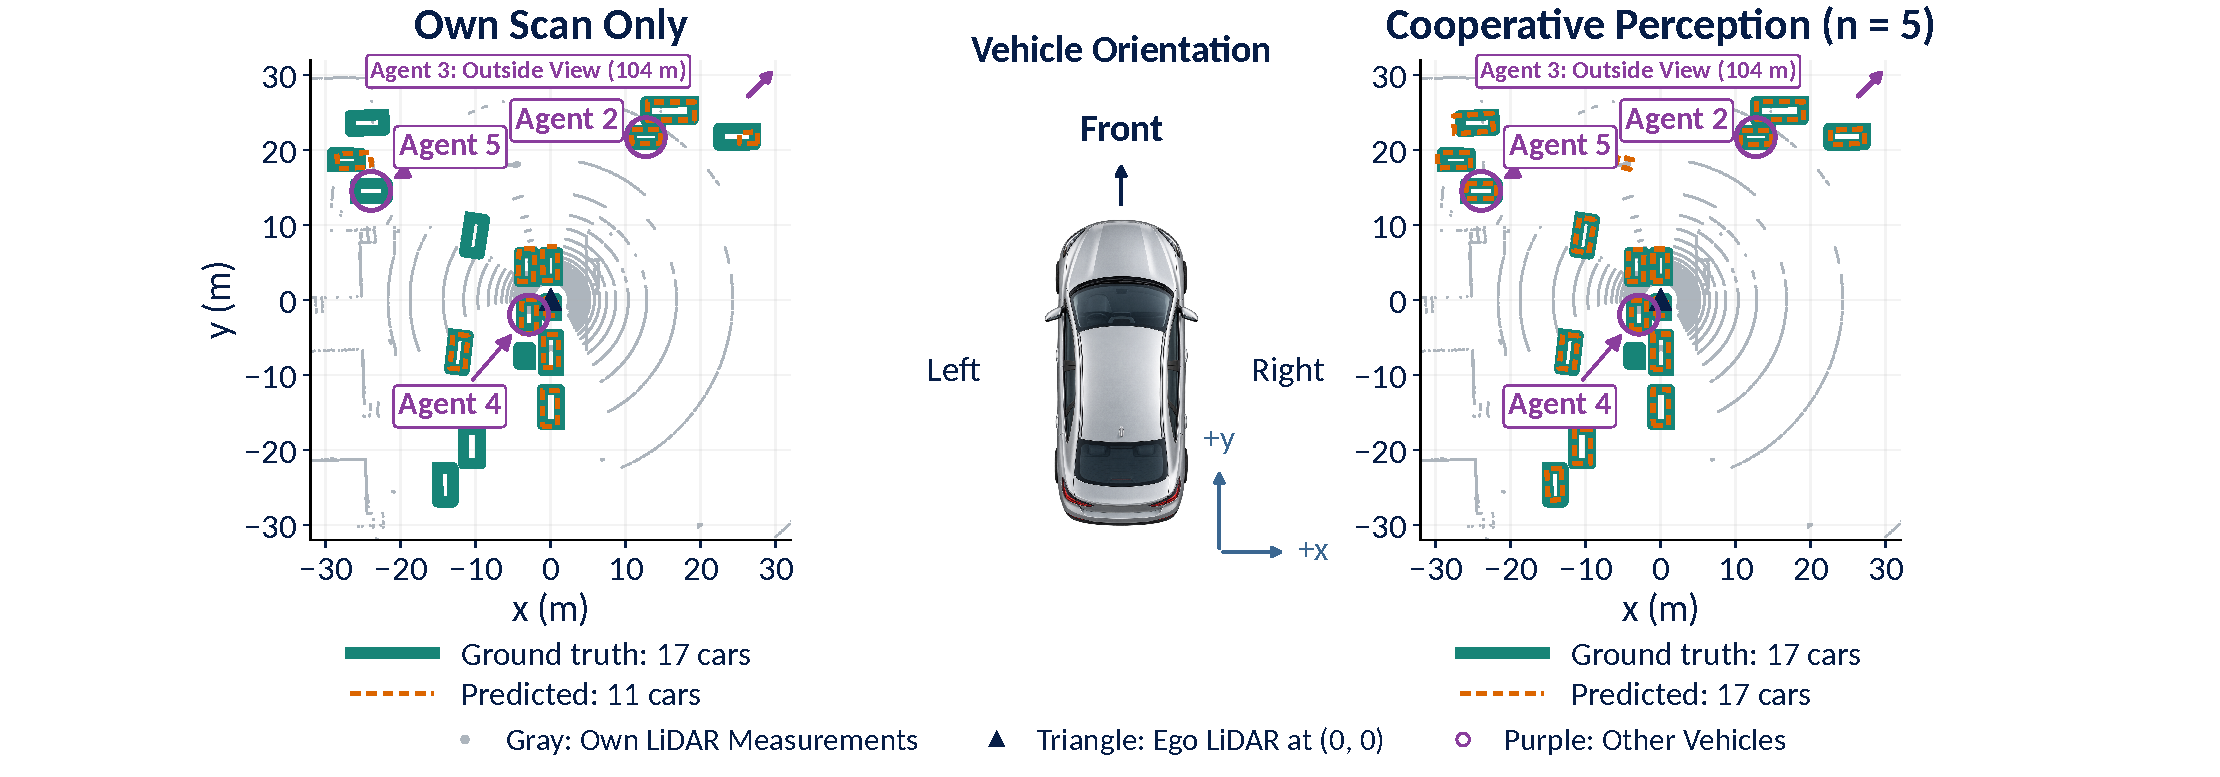
\includegraphics[width=\linewidth]{experiments/w45-2026-11-04/example-detections-v1.pdf}
\caption[Recorded local and cooperative car detections]{Recorded local and cooperative car detections in the single-frame
example. Reference and prediction outlines remain overlaid. Axes use the
vehicle-relative front-up display about the LiDAR sensor; the original
model coordinates are unchanged. The orientation icon is illustrative AI
artwork; points, reference boxes, and predictions are recorded data.}
\label{fig:detections}
\end{figure}

The example illustrates why sharing can help: another viewpoint can supply
useful features where the receiver's own observation is incomplete.
Its counts do not measure full-test AP or the performance of all five
receivers. The camera views in the slide appendix provide synchronized
context, but camera and LiDAR positions differ and the model does not use
those images as detector inputs.

\begin{figure}[htbp]
\centering
\begin{minipage}[t]{0.32\linewidth}
\centering\small\textbf{Front left}\par\smallskip
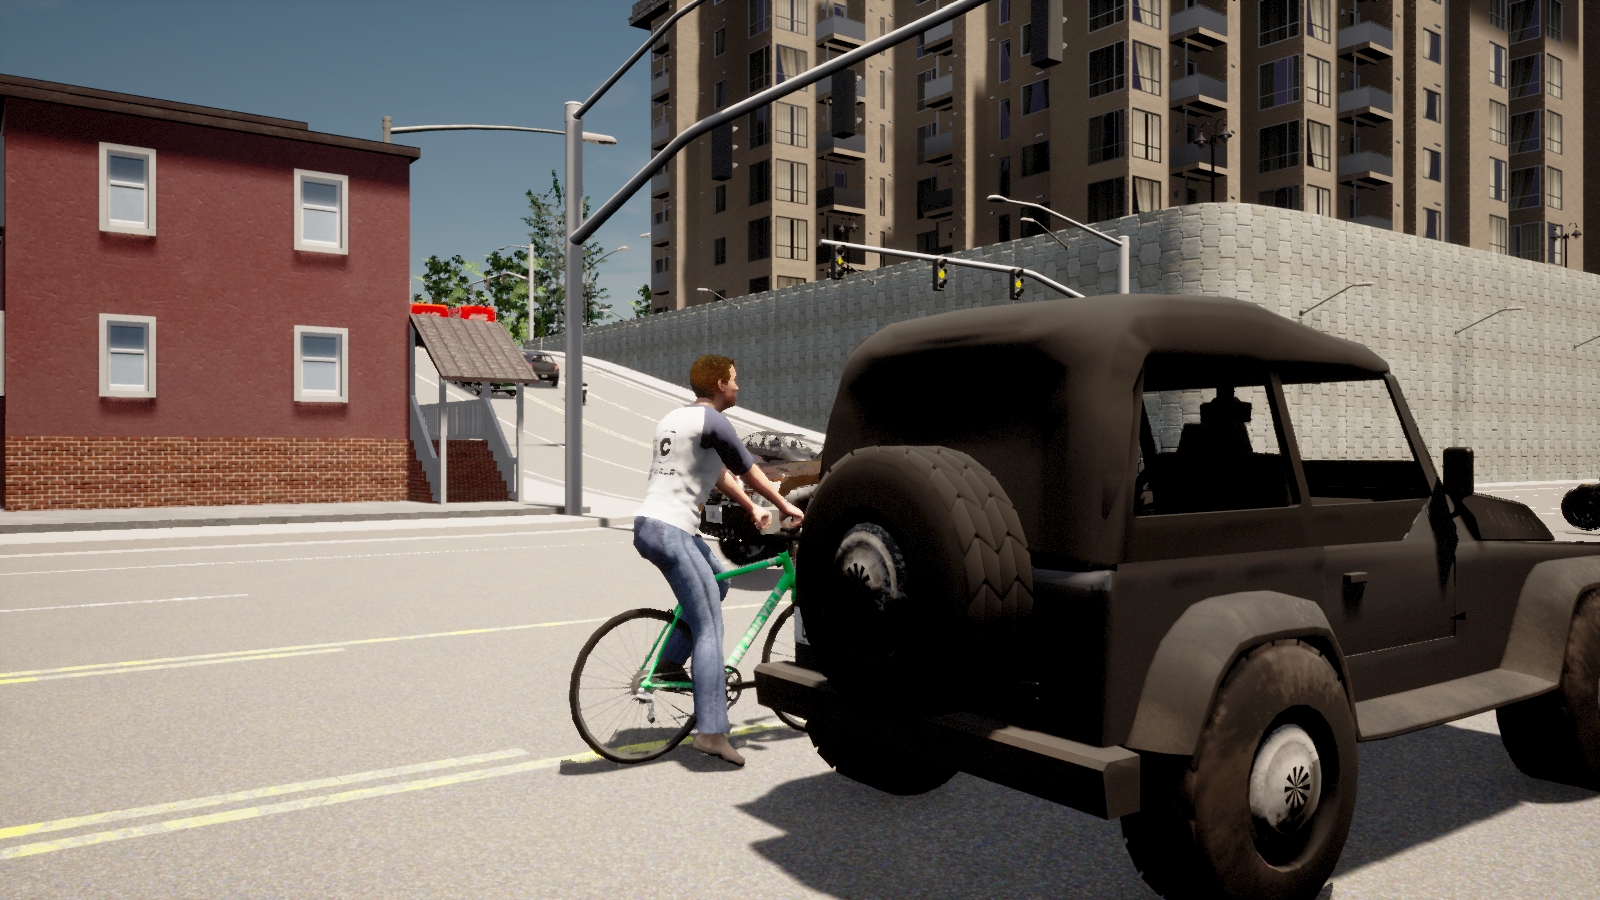
\includegraphics[width=\linewidth]{cameras/example-camera-front-left-v1.jpg}
\end{minipage}\hfill
\begin{minipage}[t]{0.32\linewidth}
\centering\small\textbf{Front}\par\smallskip
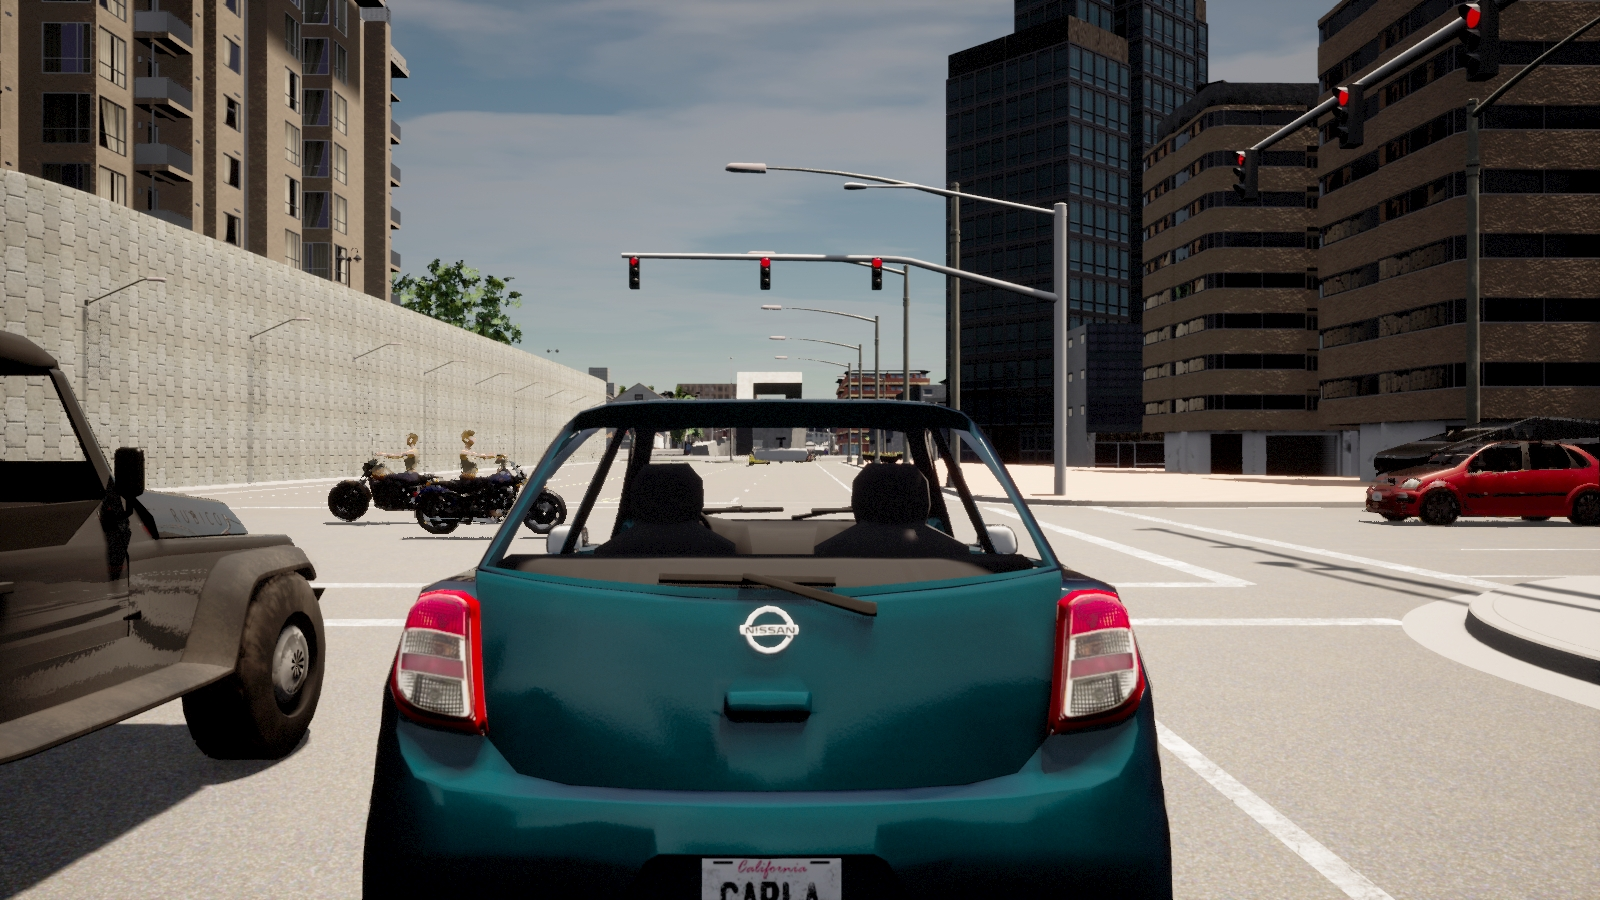
\includegraphics[width=\linewidth]{cameras/example-camera-front-v1.jpg}
\end{minipage}\hfill
\begin{minipage}[t]{0.32\linewidth}
\centering\small\textbf{Front right}\par\smallskip
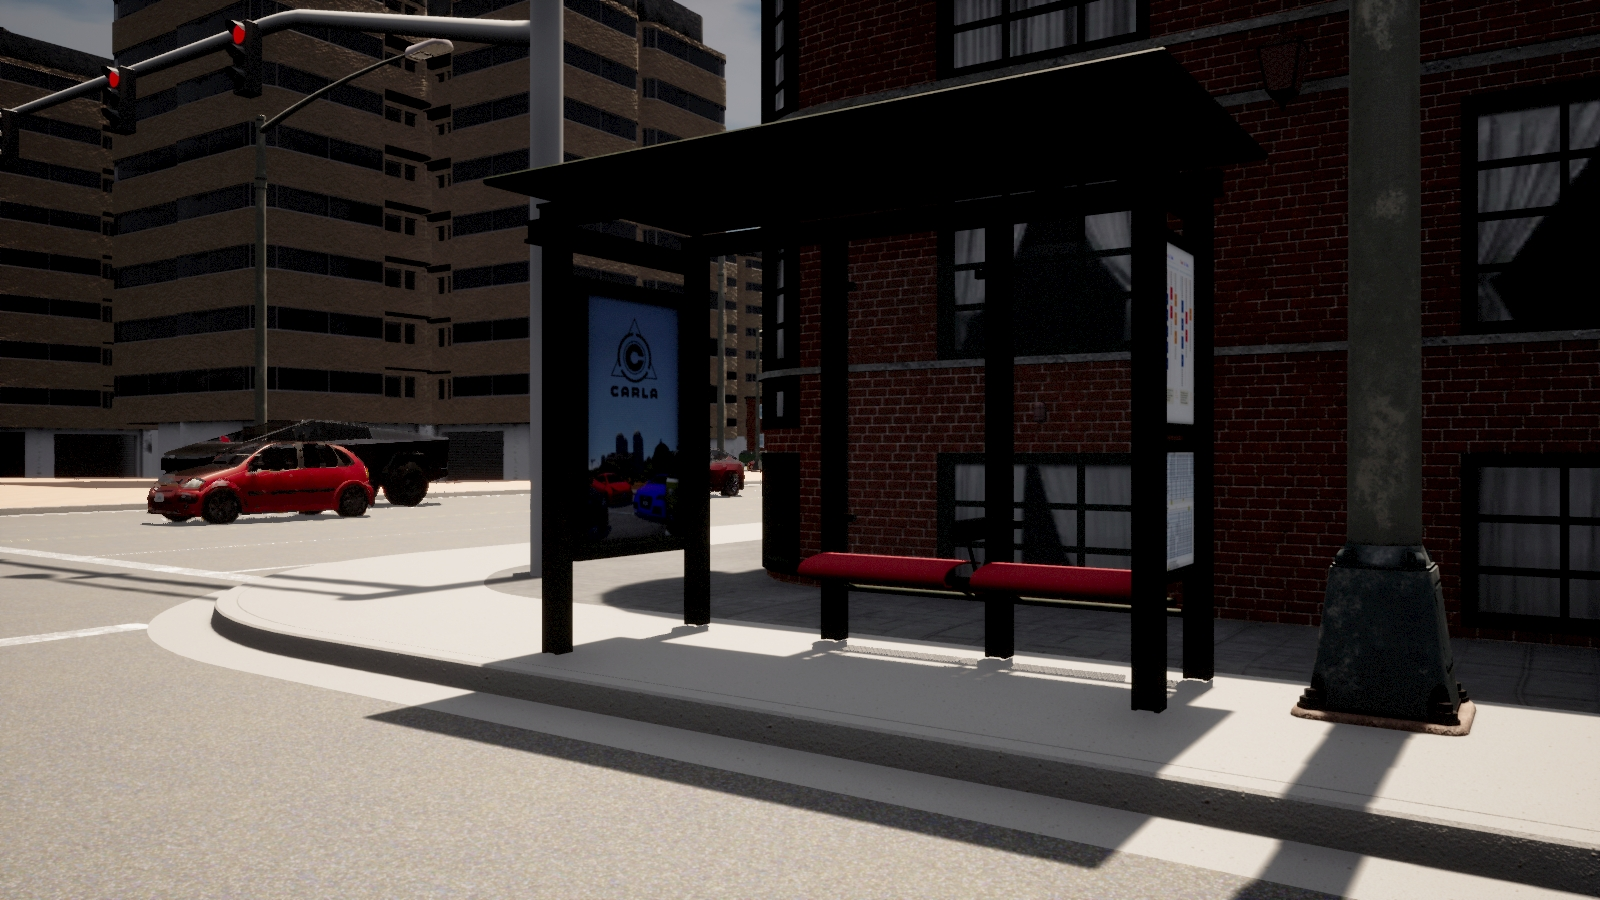
\includegraphics[width=\linewidth]{cameras/example-camera-front-right-v1.jpg}
\end{minipage}\par\medskip
\begin{minipage}[t]{0.32\linewidth}
\centering\small\textbf{Rear left}\par\smallskip
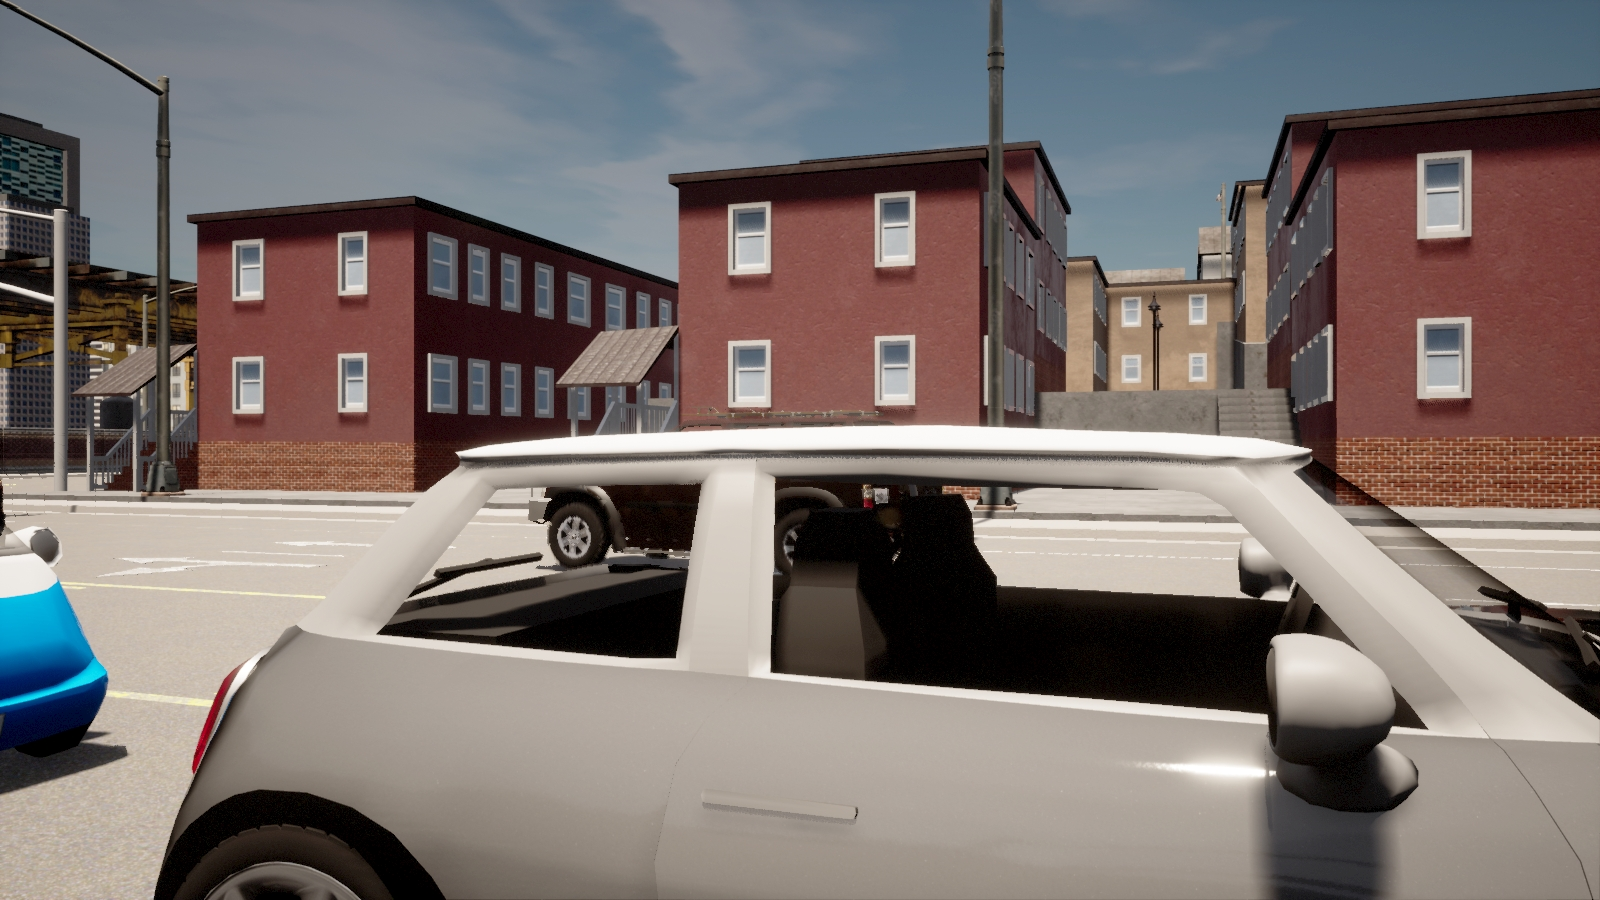
\includegraphics[width=\linewidth]{cameras/example-camera-back-left-v1.jpg}
\end{minipage}\hfill
\begin{minipage}[t]{0.32\linewidth}
\centering\small\textbf{Rear}\par\smallskip
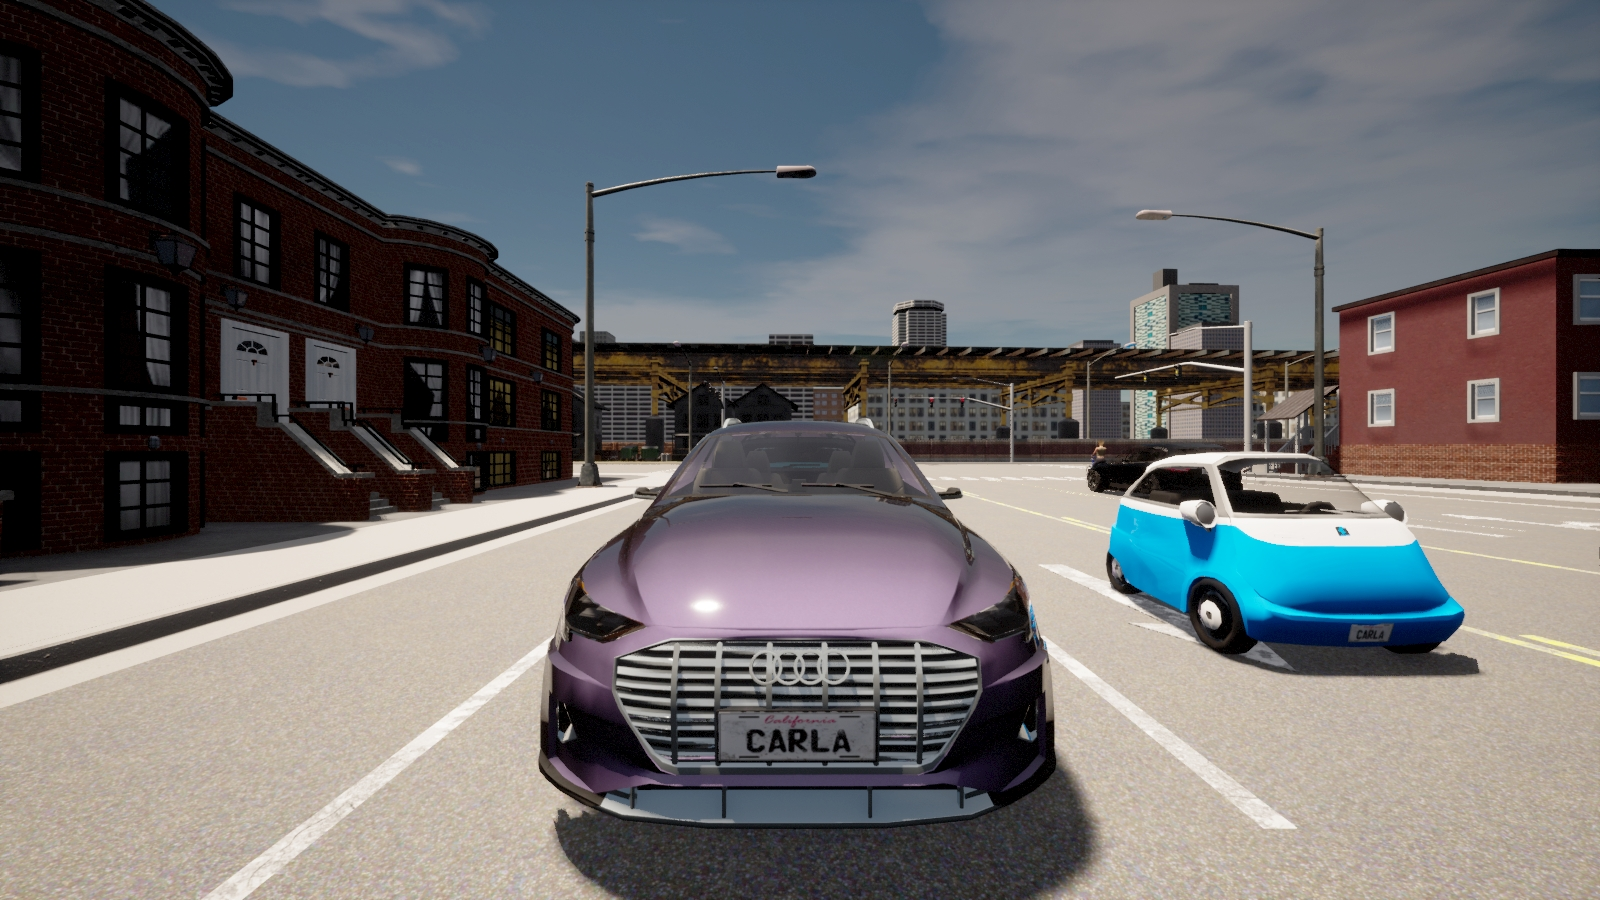
\includegraphics[width=\linewidth]{cameras/example-camera-back-v1.jpg}
\end{minipage}\hfill
\begin{minipage}[t]{0.32\linewidth}
\centering\small\textbf{Rear right}\par\smallskip
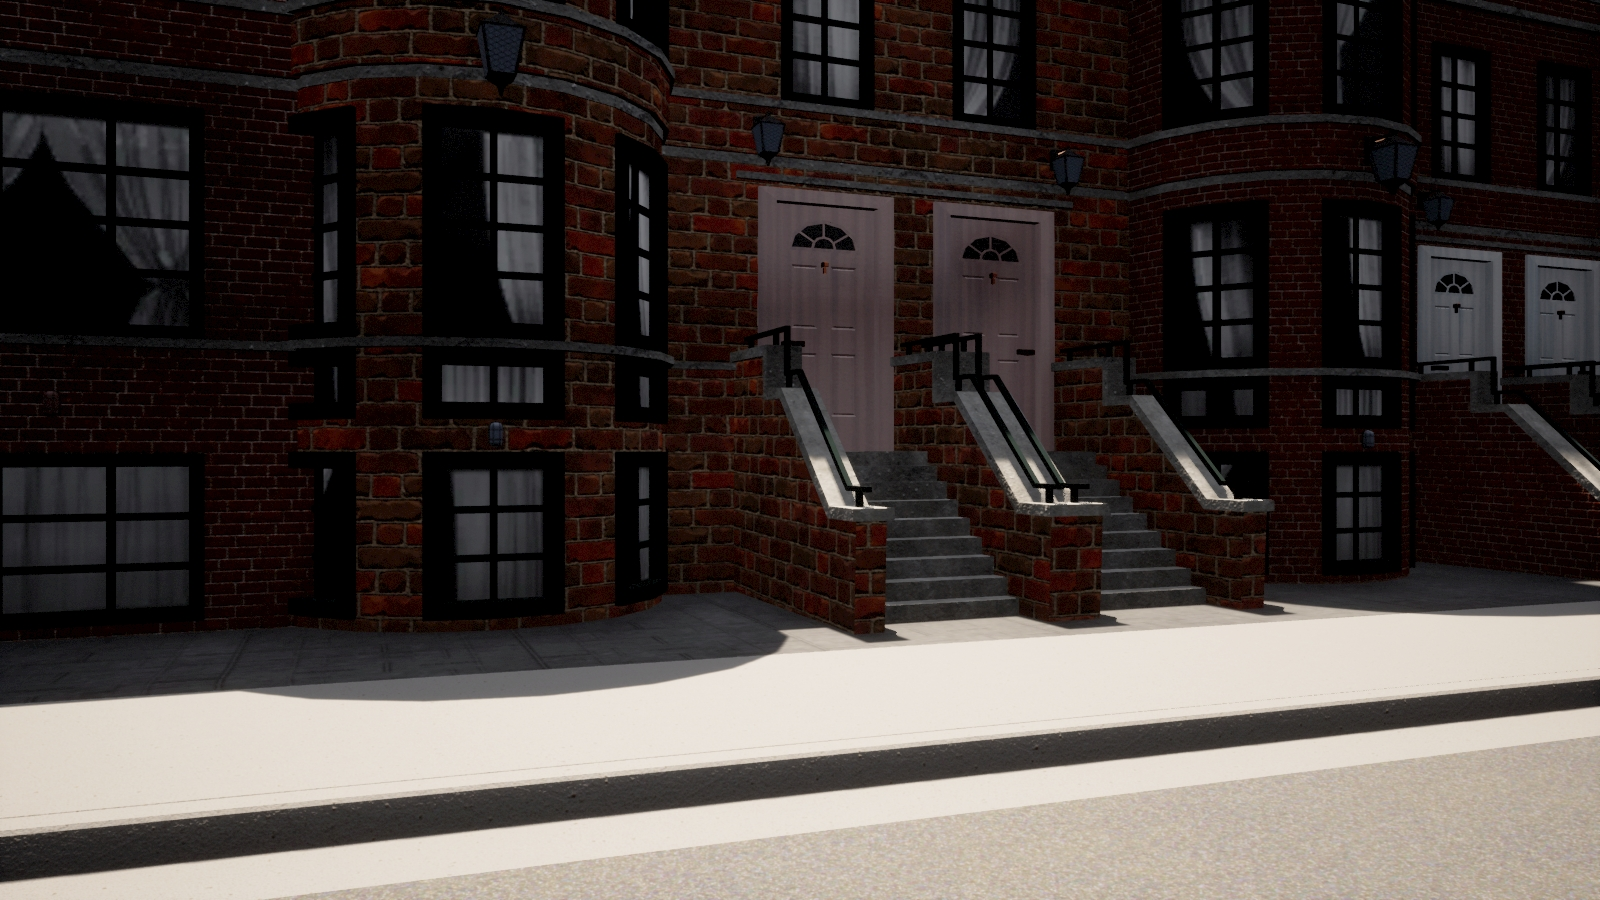
\includegraphics[width=\linewidth]{cameras/example-camera-back-right-v1.jpg}
\end{minipage}
\caption[Six synchronized camera views of the detection example]{The six
V2X-Sim 2.0 camera views archived with the project's \texttt{scene\_5},
frame \texttt{000066} example. They show the surrounding road geometry and
traffic from the ego vehicle.}
\label{fig:example-cameras}
\end{figure}

Figure~\ref{fig:example-cameras} provides the visual setting for the
bird's-eye detection overlays. The views explain why a nearby vehicle and
a farther reference box can have different visibility from the ego sensor.
They also show why the reference-box set should not be equated with the
returns visible in one scan. Camera and LiDAR mounting positions differ,
so the camera panels supply scene context rather than a pixel-level
projection of every LiDAR point.

The useful comparison in Figure~\ref{fig:detections} is therefore which
reference boxes gain a sufficiently overlapping prediction when sharing
is enabled, rather than whether the scene looks busier or the output
contains more boxes. The 10-to-16 increase in matched references supports
that interpretation for this example. Aggregate AP is still determined by
the full ranked evaluation, including false positives and missed references.

\section{Runtime Scaling with Model Input Count}
\label{sec:scaling}
\subsection{Recorded Inputs and Replay Workloads}
The runtime-only experiment fixes the checkpoint and a 30-frame cohort while
varying $n$ from one to twenty~\cite{recordruntime}. Every frame provides five
recorded vehicle inputs. For $n\leq5$, ego 1 is kept and the nearest recorded
vehicles are added. For $n>5$, the same five scans and their recorded pairwise
poses are cycled into additional tensors and active slots. For example,
$n=20$ contains four copies of the five recorded inputs.

Consequently, $n$ denotes model input slots. Above five, this experiment tests
computational load rather than perception from newly observed vehicles. No
AP or box postprocessing is computed in this runtime-only sweep. Its role is
to expose execution cost under increasing workload, not to predict detection
gains with twenty independent vehicles.

\begin{table}[htbp]
\centering
\caption{Input reuse and original fine-pair workload at selected slot counts.}
\label{tab:replay-workload}
\begin{ReportTable}{rrrL}
\ReportTableHead
\ReportTH{Slots $n$} & \ReportTH{Distinct recorded inputs} & \ReportTH{Ordered pairs $n^2$} & \ReportTH{Input composition} \\
1 & 1 & 1 & Ego input \\
5 & 5 & 25 & Five recorded inputs \\
10 & 5 & 100 & Two cycles of the five inputs \\
20 & 5 & 400 & Four cycles of the five inputs \\
\end{ReportTable}
\end{table}

Table~\ref{tab:replay-workload} makes the workload increase explicit. The
implementation allocates additional tensors and active slots even when
the underlying scan is repeated. Encoding, pairwise collaboration, and
decoding therefore process a larger group. Cycling recorded poses keeps
each replay tied to its source observation, rather than placing a newly
observed vehicle at an invented location.

\subsection{Timing Boundary}
Each condition uses the same 30 frames in three trials, with twenty warmup
forwards per condition and trial. Condition order is shuffled with seed zero.
This gives 90 timed samples per $n$, or 1,800 timed forwards and 1,200 warmup
forwards across the sweep. Inputs are already on the GPU, and CUDA is
synchronized before and after each measured forward.

The forward timer includes the encoder, pairwise fusion, decoder, and
detection heads for the \emph{entire $n$-slot group}. It excludes file reads,
CPU packing, raw LiDAR preprocessing, input transfer, model loading, warmups,
and output checks. These times are not per-vehicle wireless latency and are
not the duration of the whole data-loading/evaluation pipeline.

\subsection{Results}
Median full-group forward time increases from \ReportRuntimeStart\ ms at
$n=1$ to \ReportRuntimeEnd\ ms at $n=20$, a factor of
\ReportRuntimeFactor. Table~\ref{tab:runtime} reports every condition, with
the 95th percentile (P95) of its 90 timing samples. P95 describes the observed
tail of those timings; it is not a confidence interval for the median.

\begin{table}[htbp]
\centering
\caption{Runtime-only sweep on the fixed 30-frame cohort. The rule after
$n=5$ marks the change from distinct recorded inputs to replayed-input
workloads. Timings refer to full-group forward execution.}
\label{tab:runtime}
\input{runtime-table.generated}
\end{table}

\begin{figure}[htbp]
\centering
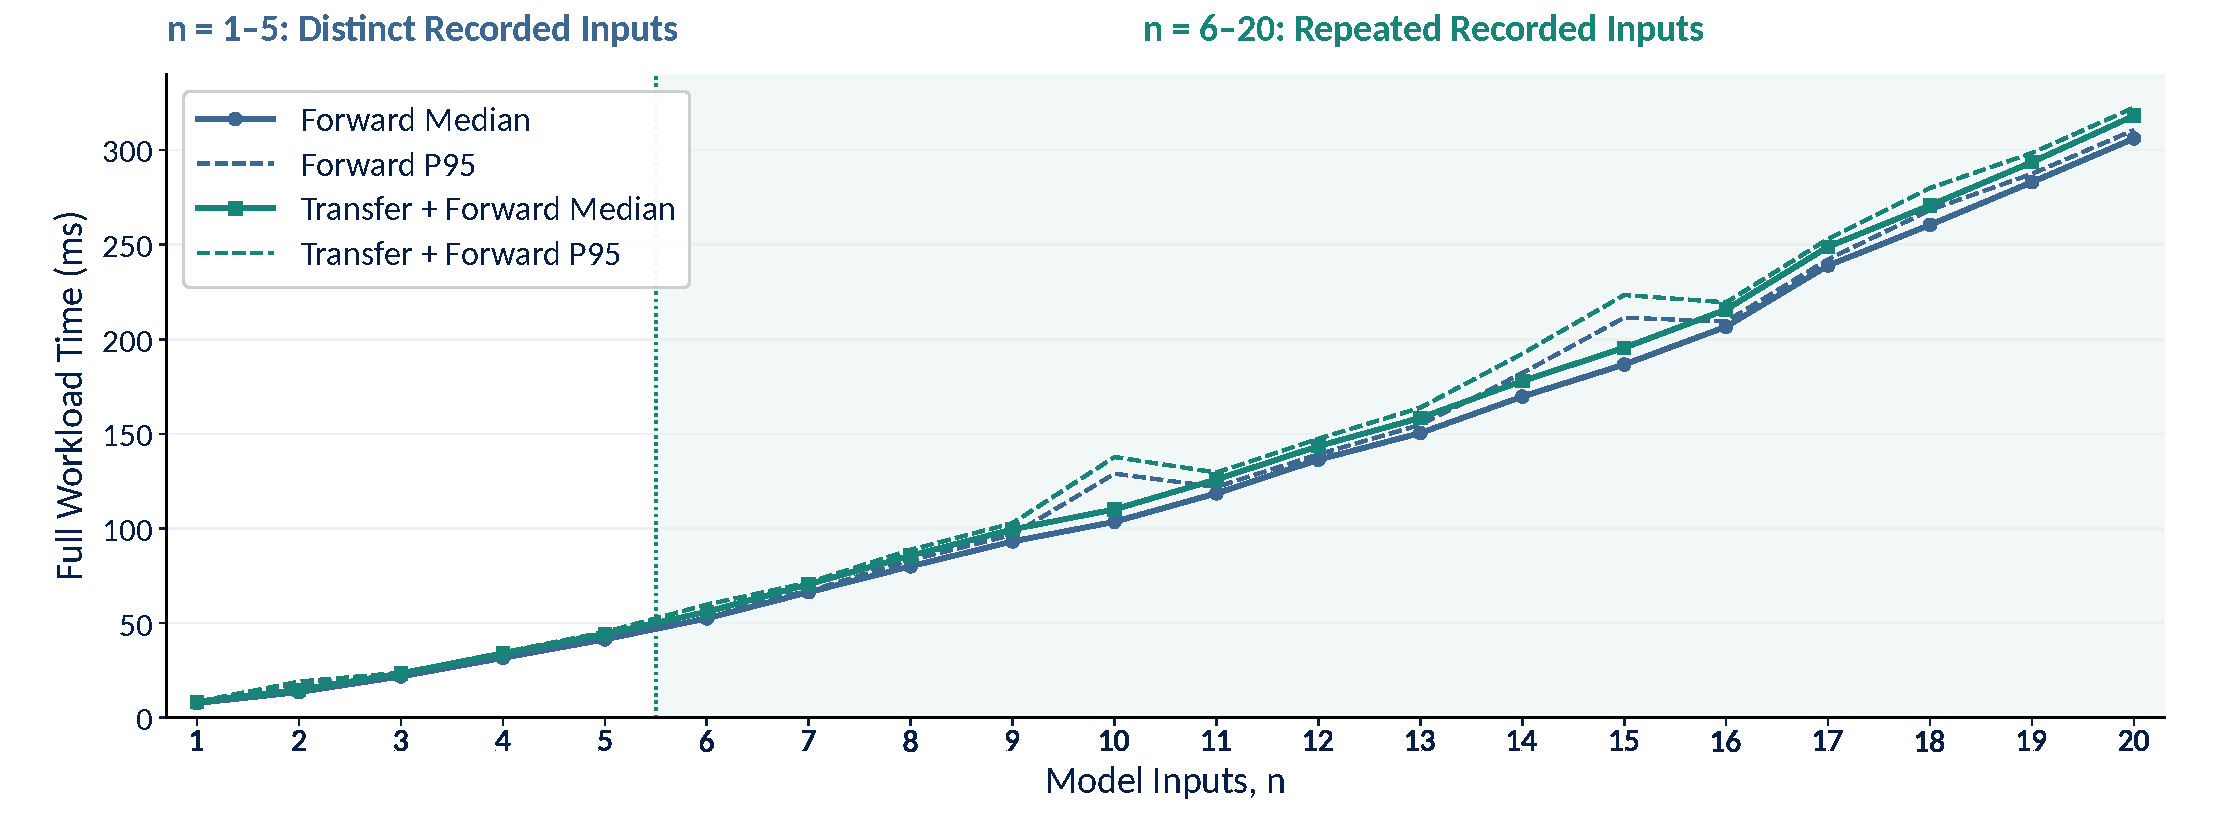
\includegraphics[width=\linewidth]{experiments/w45-2026-11-04/runtime-scaling-v1.pdf}
\caption[Recorded runtime scaling from one to twenty slots]{Saved
runtime-scaling figure. Forward timings and transfer-plus-forward
timings have different boundaries; only the former are tabulated in
Table~\ref{tab:runtime}. The plot retains the original measured medians and
P95 values~\cite{recordruntime}.}
\label{fig:runtime}
\end{figure}

The growth is consistent with the increasing cost of a pipeline containing
all-pair feature collaboration. At $n=20$, the original graph evaluates
400 ordered fine-resolution pairs including self pairs, compared with one
at $n=1$. The measured runtime ratio is not required to equal the pair-count
ratio because other stages, batching, and hardware behavior also contribute.
The experiment does not fit a universal complexity law or isolate fusion
time from the rest of the model.

The two timing boundaries in Figure~\ref{fig:runtime} are part of the
experiment setup. The forward-only series matches the tabulated GPU-ready
workload. The transfer-plus-forward series includes an additional input
transfer stage. Neither includes all operations of the full-test evaluation,
such as file access, prediction export, and AP calculation. Separating
these boundaries avoids attributing the whole evaluation duration to the
network's forward pass.

\section{Original versus Tree Collaboration}
\label{sec:tree}
\subsection{Coarse Attention and Maximum Spanning Tree}
The second custom experiment asks whether restricting expensive
fine-resolution collaboration reduces execution time and how much detection
quality is lost. The released weights are reused without retraining
\cite{recordtree}. The variant has three stages:
\begin{enumerate}
  \item \textbf{Coarse scoring.} Each $32\times32$ feature map is pooled to
    $4\times4$. All ordered pairs are aligned and scored at this coarse
    resolution, with weights normalized over senders. Each directional
    attention map is reduced to its mean squared attention.
  \item \textbf{Tree selection.} The two directional scores of an unordered
    vehicle pair are averaged. Descending Kruskal selection keeps the
    highest-scoring links that do not create a cycle, until $n-1$ remain.
    This is a maximum spanning tree, rather than a minimum spanning tree.
  \item \textbf{Fine fusion.} Each selected edge is used in both directions,
    and every self pair is retained. The original $32\times32$ alignment and
    scoring are applied only to these pairs. Attention is renormalized over
    the retained senders, and the normal decoder and heads follow.
\end{enumerate}

For each receiver--sender pair, the coarse attention statistic can be written
as
\[
 q_{u\to v}=\frac{1}{H_cW_c}\sum_{r,c}a^{\mathrm{coarse}}_{u\to v}(r,c)^2,
 \qquad q_{\{u,v\}}=\frac{q_{u\to v}+q_{v\to u}}{2},
 \quad H_c=W_c=4.
\]
The undirected tree determines which directed fine interactions are retained.
Fine pair evaluations change from $n^2$ to
\[
 n+2(n-1)=3n-2.
\]
At $n=15$, that is 225 original fine pairs versus 43 tree fine pairs, in
addition to the tree variant's 225 coarse pairs. Only the fine-pair count
becomes linear. Coarse scoring remains quadratic, and CPU Kruskal selection
introduces additional work. This is not a claim of linear complexity for the
complete algorithm.

There is one fusion round. A receiver can use its immediate tree neighbors,
but a path in the spanning tree does not transmit every remote vehicle's
features across multiple hops during that round. Sparsity therefore changes
the available information as well as the amount of computation.

\begin{figure}[htbp]
\centering
\begingroup
\colorlet{MoverCyan}{ReportCyan}
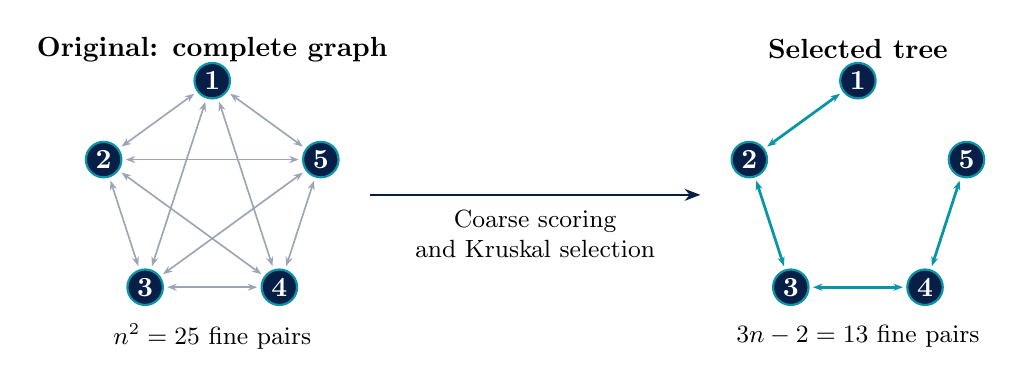
\begin{tikzpicture}[font=\small]
  \node[font=\bfseries] at (2,4.0) {Original: complete graph};
  \node[font=\bfseries] at (10.2,4.0) {Selected tree};
  \foreach \Agent in {1,...,5} {
    \pgfmathsetmacro{\Angle}{90+360*(\Agent-1)/5}
    \coordinate (full-node-\Agent) at
      ({2+1.45*cos(\Angle)},{2.15+1.45*sin(\Angle)});
    \coordinate (tree-node-\Agent) at
      ({10.2+1.45*cos(\Angle)},{2.15+1.45*sin(\Angle)});
  }
  \foreach \Sender in {1,...,5} {
    \foreach \Receiver in {1,...,5} {
      \ifnum\Sender<\Receiver
        \draw[{Stealth[length=1.2mm]}-{Stealth[length=1.2mm]},
          draw=ReportNavy!40,line width=0.6pt,
          shorten <=8pt,shorten >=8pt]
          (full-node-\Sender) -- (full-node-\Receiver);
      \fi
    }
  }
  % The saved n=5 preflight links from the versioned topology-example.tex.
  \foreach \From/\To in {3/4,1/2,2/3,4/5} {
    \draw[{Stealth[length=1.2mm]}-{Stealth[length=1.2mm]},
      draw=ReportCyan,line width=1pt,shorten <=8pt,shorten >=8pt]
      (tree-node-\From) -- (tree-node-\To);
  }
  \foreach \Agent in {1,...,5} {
    \foreach \Prefix in {full,tree} {
      \node[circle,fill=ReportNavy,draw=ReportCyan,line width=0.8pt,
        minimum size=0.45cm,inner sep=0pt,text=white,font=\bfseries]
        at (\Prefix-node-\Agent) {\Agent};
    }
  }
  \draw[-{Stealth[length=2mm]},draw=ReportNavy,line width=0.9pt]
    (4.0,2.15) -- (8.2,2.15);
  \node[align=center] at (6.1,1.65) {Coarse scoring\\and Kruskal selection};
  \node at (2,0.35) {$n^2=25$ fine pairs};
  \node at (10.2,0.35) {$3n-2=13$ fine pairs};
\end{tikzpicture}
\endgroup

\caption[Complete collaboration and the saved five-slot tree]{The project
topology diagram adapted for the report, using the saved five-slot preflight
tree. Double arrows denote interactions in both directions. Self links
are counted in the computation but omitted from the drawing. The original
has 25 fine pairs; the tree has 13 fine pairs plus coarse scoring.}
\label{fig:tree-topology}
\end{figure}

Figure~\ref{fig:tree-topology} gives a concrete example of what a receiver
loses when edges are removed. In the displayed tree, node 1 has node 2 as
its only peer neighbor. Its fine fusion can combine the self contribution
and node 2, while the original graph can use all five inputs. Node 3 has
two peer neighbors and can combine those with its own features. A path
from node 1 to node 5 establishes graph connectivity, but it does not
make node 5's original map an immediate input to node 1 in one fusion round.

The displayed topology is one saved preflight example. Selection is driven
by the coarse attention scores of the evaluated input group; the figure
does not assign a fixed chain to every frame. It illustrates the difference
between retaining connectivity and retaining all direct fine observations.

\subsection{Matched Timing and Accuracy Protocol}
The comparison uses the same 30 ego-1 views from three recorded test scenes
at every condition, with 427 reference car boxes counted once across the
cohort. Both methods use the unchanged checkpoint, float32 precision, and
the same retained-prediction settings. There are three timing trials and 90
samples per method and $n$, covering $n=1,\ldots,15$. The specification records
twenty warmups per method/count/trial, shuffled condition order with seed
zero, deterministic cuDNN, and TF32 disabled.

The timer includes the complete model, coarse scoring, CPU tree selection,
fine fusion, decoder, and heads. Inputs are already on the GPU. Reads and
packing, transfers, warmups, model loading, box decoding, NMS, and AP scoring
are outside the forward timer. AP is evaluated separately on the original
ego-1 labels. The run contains 2,700 timed forwards in total, and recorded ego
outputs are identical across timing trials for a given condition.

As in the runtime-only workload, $n\leq5$ uses distinct recorded inputs,
while larger $n$ replays the five recorded scans and poses. AP above five
describes the behavior of those repeated inputs, not the benefit of extra
independently recorded viewpoints.

\subsection{Complete Results and Trade-Off}
Table~\ref{tab:tree} reproduces all fifteen measured conditions from the
versioned CSV and checks them against the saved JSON during report builds.
The AP values are percentages; differences between them are percentage points.

\begin{table}[htbp]
\centering
\caption{Matched Original/Tree comparison on 30 ego-1 views. Below the rule
after $n=5$, additional slots replay the five recorded inputs. The table is
separate from the full-test benchmark and the runtime-only sweep.}
\label{tab:tree}
\input{tree-table.generated}
\end{table}

At $n=15$, median time falls from \ReportOriginalTime\ to \ReportTreeTime\ ms,
a \ReportTreeReduction\% reduction. AP@0.5 decreases from
\ReportOriginalAPFifty\% to \ReportTreeAPFifty\%, a loss of
\ReportTreeDropFifty\ percentage points. AP@0.7 decreases from
\ReportOriginalAPSeventy\% to \ReportTreeAPSeventy\%, a loss of
\ReportTreeDropSeventy\ points. This is a substantial runtime reduction
accompanied by a substantial accuracy loss, rather than an improvement at
unchanged detection quality.

The same trade-off is visible within the distinct-input region. At $n=5$,
median time falls from 41.57 to 36.54 ms, while AP@0.5 falls from 74.46\% to
62.65\% and AP@0.7 from 67.53\% to 53.66\%. Thus the accuracy penalty is not
only an artifact of replaying inputs above five.

At $n=1$ and $n=2$, the original and tree graphs coincide, and the saved
predictions are identical. Small differences in their medians are timing
variation, not evidence of a useful speed or accuracy difference. At larger
$n$, the original AP is not strictly monotonic, and replay does not create
new information. No general claim that increasing slots must improve
detection follows from the table.

\section{Discussion and Limitations}
The full-test comparison establishes that feature sharing benefits the
evaluated pretrained student under the stated conditions. It holds model
weights fixed and changes collaboration availability. It does not determine
the ranking of separately trained local, early-fusion, and intermediate-fusion
models. In particular, the planned early-fusion baseline remains unmeasured.

The scaling experiments address a different question: whether complete
collaboration is computationally expensive as the number of slots increases,
and what happens when its fine interactions are restricted. The tree ablation
shows a measured runtime--accuracy trade-off. Removing fine edges can reduce
access to complementary observations in a single fusion round. This is a
plausible explanation of the AP loss, consistent with the mechanism, rather
than a measured causal decomposition of every missed detection.

Several limits constrain these conclusions:
\begin{itemize}
  \setlength{\itemsep}{0pt}
  \setlength{\parsep}{0pt}
  \item \textbf{Ideal communication and poses.} The experiments do not vary
    latency, packet loss, bandwidth limits, asynchronous sensing, or pose
    errors. Their forward times cannot be used directly as wireless latency.
  \item \textbf{Replay beyond five inputs.} Larger workloads increase active
    model slots without adding independent viewpoints or real vehicles.
  \item \textbf{Different evaluation populations.} The full-test AP pools
    4,000 active views; the tree AP uses 30 fixed ego views. Their numerical
    levels are not interchangeable estimates of the same population.
  \item \textbf{One checkpoint and device.} No retraining, model-family
    comparison, multi-GPU experiment, or cross-hardware generalization is
    established. The sparse graph was not trained to compensate for missing
    fine links.
  \item \textbf{Limited uncertainty analysis.} Repeated timings characterize
    runtime variation on a fixed cohort. They do not create new independent
    detection samples, and no confidence interval for population AP is
    reported.
  \item \textbf{Version and scope.} The evaluation uses V2X-Sim 2.0, unlike
    the original paper's 1.0 benchmark. Fixed-checkpoint losses are not a
    training history or evidence about convergence.
\end{itemize}

Follow-up experiments could hold the evaluation population and postprocessing
fixed while varying retained neighbors, selection resolution, and fusion
rounds. Further recordings would allow study beyond five independent
vehicles. Fine-tuning a sparse student and testing communication impairments
would require new training and an explicit transport model, respectively.

\section{Conclusion}
DiscoNet combines per-vehicle feature extraction, pose-based alignment,
spatial attention, and decoder skip connections to produce cooperative car
detections. On the complete prepared V2X-Sim 2.0 test split, enabling sharing
in the same student raises AP by \ReportGainFifty\ and \ReportGainSeventy\
percentage points at IoU 0.5 and 0.7. This directly answers the completed
own-scan/cooperative comparison under ideal conditions.

The separate workload sweep shows increasing full-group computation as
model input count grows. The matched tree experiment reduces fine pair
evaluations but also reduces detection quality: at 15 slots, median runtime
is \ReportTreeReduction\% lower, with AP losses of \ReportTreeDropFifty\ and
\ReportTreeDropSeventy\ points. The results support studying collaboration
sparsity as a trade-off, while preserving the distinction between additional
computation and additional independently observed information.

\cleartorecto
\appendix
\section{Reusable Blocks and Convolution Detail}
\label{app:implementation}
The slide appendix presents the architecture through callable PyTorch-style
blocks. The following excerpt preserves that decomposition; it explains the
forward structure rather than replacing the authors' implementation.

\subsection{Callable Units and Shape Contracts}

\begin{lstlisting}
def norm_relu(c):
    return nn.Sequential(nn.BatchNorm2d(c), nn.ReLU())

def unit_2d(c_in, r, c_out):
    conv = nn.Conv2d(c_in, c_out, 3, stride=r, padding=1)
    return nn.Sequential(conv, *norm_relu(c_out))

def unit_2d_initial(c_in, c_out):
    return unit_2d(c_in, 1, c_out)

def unit_2d_keep(c_in):
    return unit_2d(c_in, 1, c_in)

def unit_2d_down(c_in):
    return unit_2d(c_in, 2, 2*c_in)

def decoder_block(c_in, c_out):
    return nn.Sequential(unit_2d_initial(c_in, c_out),
                         unit_2d_keep(c_out))

def upsample_concat(decoder_features, skip_features):
    upsampled_features = F.interpolate(
        decoder_features, scale_factor=2, mode="nearest")
    return torch.cat((upsampled_features, skip_features), dim=1)
\end{lstlisting}

For even input dimensions, an Initial or Keep unit preserves spatial
resolution, while a Down unit halves height and width. More generally, the
kernel-3, padding-1, stride-$r$ convolution gives
$H_{\mathrm{out}}=\lfloor(H_{\mathrm{in}}-1)/r\rfloor+1$, with the analogous
formula for width. The attention pointwise unit instead uses a $1\times1$
convolution to change channels without mixing neighboring spatial cells.
Normalization and activation preserve the tensor shape.

An encoder stage composes two 2D units and, where specified, a pointwise 3D
unit. In this single-frame reconstruction, the 3D helper temporarily inserts
a singleton depth axis, applies a $1\times1\times1$ Conv3d, and flattens that
axis again. It preserves the displayed $H/W/C$ dimensions. Its name is not
evidence of multi-frame temporal aggregation in this forward path.

\noindent\begin{minipage}{\linewidth}
\subsection{The Alignment Code Example}
The project illustrates spatial alignment with a square feature map and a
rotation followed by translation. The excerpt below is the existing
teaching implementation used beside Figure~\ref{fig:rotation-translation}.
It constructs a forward transform, inverts it for output-to-input sampling,
and applies the same grid to every channel.

\lstinputlisting[firstline=4]{assets/final/graph/feature_alignment_example_v1.py}
\end{minipage}

The example's $x$ coordinate points right and $y$ points down. Translation
is expressed in cells of this small feature grid. The factors $2/W$ and
$2/H$ convert displacements to the normalized grid coordinates used by
the sampler. The example call is
\begin{lstlisting}
aligned_features = align_features(
    sender_features, angle_deg=90, dx=1, dy=1)
\end{lstlisting}
The original model's pose handling and scale conversion remain part of
its implementation; this small example isolates the sampling operation.

\FloatBarrier
\subsection{Numerical Input and Kernel Dimensions}
The separate convolution walkthrough uses a video tensor with three frames,
three channels, height three, and width four. Figure~\ref{fig:conv-input}
shows all values. Channel colors remain fixed across frames, making it
possible to track a spatial patch through the numerical calculation.

\begin{figure}[htbp]
\centering
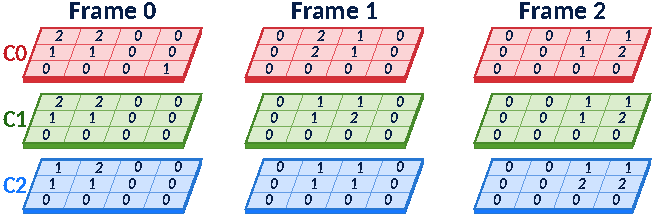
\includegraphics[width=\linewidth]{convolution/conv-palette-v2-inputs.pdf}
\caption[The three-frame, three-channel convolution input]{The project's
numerical tensor example. Columns are frames; colors distinguish channels
C0, C1, and C2. Each channel plane has three rows and four columns.}
\label{fig:conv-input}
\end{figure}

\begin{figure}[htbp]
\centering
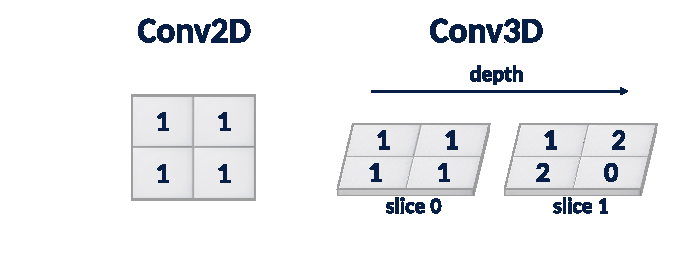
\includegraphics[width=\linewidth]{convolution/conv-palette-v2-kernels-rich-v1.pdf}
\caption[Spatial and temporal kernel slices]{Project kernel illustrations.
The Conv2D spatial kernel contains ones. The Conv3D kernel has two temporal
slices, with different weights in the second slice. Each illustrated
spatial/temporal kernel is applied across the input channels.}
\label{fig:conv-kernels}
\end{figure}

The examples use stride one, no padding, zero bias, and one output channel.
A $2\times2$ spatial kernel on a $3\times4$ plane produces a $2\times3$
output. A Conv3D kernel of depth two on three input frames also produces
two output depth slices. Its complete output shape is therefore
$2\times2\times3$ in depth--height--width order.

\FloatBarrier
\subsection{Conv2D: Accumulating Across Channels}
For one output channel, the weight tensor contains a spatial kernel for
every input channel. In this example all those Conv2D weights are one.
At the upper-left output, the four-cell patches of Frame 0 sum to 6 in
C0, 6 in C1, and 5 in C2. The contributions are added:
\[
 y_{0,0}=
 \underbrace{(2+2+1+1)}_{\mathrm{C0}}+
 \underbrace{(2+2+1+1)}_{\mathrm{C1}}+
 \underbrace{(1+2+1+1)}_{\mathrm{C2}}=17.
\]

\begin{figure}[htbp]
\centering
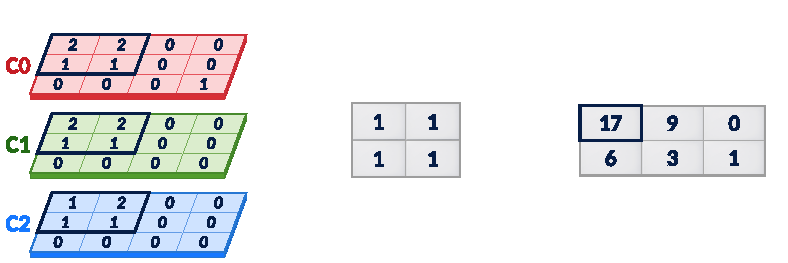
\includegraphics[width=\linewidth]{convolution/conv-palette-v2-conv2d-r0c0-rich-v1.pdf}
\caption[The first Conv2D output and the complete spatial result]{Project
Conv2D example. Outlines select the upper-left patch in each channel;
the highlighted output sums all channel contributions.}
\label{fig:conv2d-example}
\end{figure}

Sliding the same kernel across Frame 0 gives
\[
 \begin{bmatrix}17&9&0\\6&3&1\end{bmatrix}.
\]
The output is one channel because all three input-channel contributions
feed the same filter. Multiple output channels would use additional learned
filters. Convolving each frame separately does not mix the values of
Frame 0 with those of Frame 1.

\FloatBarrier
\subsection{Conv3D: Accumulating Across Time and Channels}
The temporal kernel in Figure~\ref{fig:conv-kernels} uses
\[
 K_0=\begin{bmatrix}1&1\\1&1\end{bmatrix},\qquad
 K_1=\begin{bmatrix}1&2\\2&0\end{bmatrix}.
\]
The same two-slice pattern is used for each input channel in this teaching
example. At output $(d,r,c)=(0,0,0)$, $K_0$ multiplies the upper-left patch
of Frame 0 and $K_1$ multiplies the corresponding patch of Frame 1. The
recorded arithmetic is
\[
 (6+4)_{\mathrm{C0}}+(6+2)_{\mathrm{C1}}+(5+2)_{\mathrm{C2}}=25.
\]
This calculation combines both temporal slices and all three channels.

\begin{figure}[htbp]
\centering
\newcommand{\ReportConvThreeRow}[3]{%
  \begin{minipage}[c]{0.57\linewidth}
    \centering\small\textbf{#1}\par\smallskip
    \includegraphics[width=\linewidth]{convolution/conv-palette-v2-conv3d-d#2r0c0.pdf}
  \end{minipage}\hfill
  \begin{minipage}[c]{0.19\linewidth}
    \centering\small\textbf{Kernel}\par\smallskip
    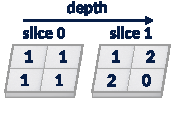
\includegraphics[width=\linewidth]{convolution/conv-palette-v2-kernel3d-rich-v1.pdf}
  \end{minipage}\hfill
  \begin{minipage}[c]{0.20\linewidth}
    \centering\small\textbf{Output: #3}\par\smallskip
    \includegraphics[width=\linewidth]{convolution/conv3d-output-parallelepipeds-v3-d#2r0c0-rich-v1.pdf}
  \end{minipage}%
}
\ReportConvThreeRow{Frames 0 and 1}{0}{$d=0$}\par\bigskip
\ReportConvThreeRow{Frames 1 and 2}{1}{$d=1$}

\caption[Two temporal positions of the Conv3D window]{The project's input
patches, temporal kernel, and output diagrams combined at their original
aspect ratios. Above, Frames 0 and 1 produce 25 at $(0,0,0)$. Below, moving
the temporal window to Frames 1 and 2 produces 8 at $(1,0,0)$.}
\label{fig:conv3d-example}
\end{figure}

Advancing the depth coordinate moves the window to Frames 1 and 2. At
$(1,0,0)$, the three channel contributions become $4+0$, $2+0$, and
$2+0$, giving eight. The complete two output slices in the saved
walkthrough are
\[
 Y_0=\begin{bmatrix}25&27&11\\14&15&5\end{bmatrix},\qquad
 Y_1=\begin{bmatrix}8&21&24\\4&16&20\end{bmatrix}.
\]
Depth and channels are separate axes: the kernel slides over time while
accumulating over channels. This genuine multi-frame example explains
the additional dimension of Conv3D. It should be distinguished from the
architecture's pointwise helper on a singleton depth axis. The complete
sequence of spatial and temporal windows remains in Appendix C of the
presentation.

\cleartorecto
\phantomsection
\addcontentsline{toc}{section}{References}
\begingroup
\small\raggedright
% Let long repository links wrap at hyphens.
\def\UrlBigBreaks{\do\-}
\bibliographystyle{plain}
\bibliography{references,final/evidence}
\endgroup
\end{document}
